% !TeX spellcheck = hu_HU
% !TeX encoding = UTF-8
% !TeX program = xelatex
\documentclass[11pt,a4paper,oneside]{report}             % Single-side
%\documentclass[11pt,a4paper,twoside,openright]{report}  % Duplex

% thanks to http://tex.stackexchange.com/a/47579/71109
\usepackage{ifxetex}
\usepackage{ifluatex}
\newif\ifxetexorluatex % a new conditional starts as false
\ifnum 0\ifxetex 1\fi\ifluatex 1\fi>0
   \xetexorluatextrue
\fi

\ifxetexorluatex
  \usepackage{fontspec}
\else
  \usepackage[T1]{fontenc}
  \usepackage[utf8]{inputenc}
  \usepackage[lighttt]{lmodern}
\fi

\usepackage[english,magyar]{babel} % Alapértelmezés szerint utoljára definiált nyelv lesz aktív, de később külön beállítjuk az aktív nyelvet.

%\usepackage{cmap}
\usepackage{amsfonts,amsmath,amssymb} % Mathematical symbols.
%\usepackage[ruled,boxed,resetcount,linesnumbered]{algorithm2e} % For pseudocodes. % beware: this is not compatible with LuaLaTeX, see http://tex.stackexchange.com/questions/34814/lualatex-and-algorithm2e
\usepackage{booktabs} % For publication quality tables for LaTeX
\usepackage{graphicx}

%\usepackage{fancyhdr}
%\usepackage{lastpage}

\usepackage{anysize}
%\usepackage{sectsty}
\usepackage{setspace} % For setting line spacing

\usepackage[unicode]{hyperref} % For hyperlinks in the generated document.
\usepackage{xcolor}
\usepackage{listings} % For source code snippets.

\usepackage[amsmath,thmmarks]{ntheorem} % Theorem-like environments.

\usepackage[hang]{caption}

\singlespacing

\newcommand{\selecthungarian}{
	\selectlanguage{magyar}
	\setlength{\parindent}{2em}
	\setlength{\parskip}{0em}
	\frenchspacing
}

\newcommand{\selectenglish}{
	\selectlanguage{english}
	\setlength{\parindent}{0em}
	\setlength{\parskip}{0.5em}
	\nonfrenchspacing
	\renewcommand{\figureautorefname}{Figure}
	\renewcommand{\tableautorefname}{Table}
	\renewcommand{\partautorefname}{Part}
	\renewcommand{\chapterautorefname}{Chapter}
	\renewcommand{\sectionautorefname}{Section}
	\renewcommand{\subsectionautorefname}{Section}
	\renewcommand{\subsubsectionautorefname}{Section}
}

\usepackage[numbers]{natbib}
\usepackage{xspace}
%\usepackage{biblatex}


% Set the main variables
\newcommand{\vikszerzoVezeteknev}{Tutkovics}
\newcommand{\vikszerzoKeresztnev}{András}

\newcommand{\vikkonzulensAMegszolitas}{dr.~}
\newcommand{\vikkonzulensAVezeteknev}{Rétvári}
\newcommand{\vikkonzulensAKeresztnev}{Gábor Ferenc}

\newcommand{\vikkonzulensBMegszolitas}{}
\newcommand{\vikkonzulensBVezeteknev}{}
\newcommand{\vikkonzulensBKeresztnev}{}

\newcommand{\vikkonzulensCMegszolitas}{}
\newcommand{\vikkonzulensCVezeteknev}{}
\newcommand{\vikkonzulensCKeresztnev}{}

\newcommand{\vikcim}{Felhő alapú alkalmazások automatikus horizontális skálázásának vizsgálata} % Cím
\newcommand{\viktanszek}{\bmetmit} % Tanszék
\newcommand{\vikdoktipus}{\msc} % Dokumentum típusa (\bsc vagy \msc)
\newcommand{\vikmunkatipusat}{diplomatervet} % a "hallgató nyilatkozat" részhez: szakdolgozatot vagy diplomatervet

% %--------------------------------------------------------------------------------------
% TDK-specifikus változók
%--------------------------------------------------------------------------------------
\newcommand{\tdkszerzoB}{Második Szerző} % Második szerző neve; hagyd üresen, ha egyedül írtad a TDK-t.
\newcommand{\tdkev}{2014} % A dolgozat írásának éve (pl. "2014") (Ez OTDK-nál eltérhet az aktuális évtől.)

% További adatok az OTDK címlaphoz (BME-s TDK-hoz nem kell kitölteni)
\newcommand{\tdkevfolyamA}{IV} % Első szerző évfolyama, római számmal (pl. IV).
\newcommand{\tdkevfolyamB}{III} % Második szerző évfolyama, római számmal (pl. III).
\newcommand{\tdkkonzulensbeosztasA}{egyetemi tanár} % Első konzulens beosztása (pl. egyetemi docens)
\newcommand{\tdkkonzulensbeosztasB}{doktorandusz} % Második konzulens beosztása (pl. egyetemi docens)

\newcommand{\szerzoMeta}{\vikszerzoVezeteknev{} \vikszerzoKeresztnev} % egy szerző esetén
%\newcommand{\szerzoMeta}{\vikszerzoVezeteknev{} \vikszerzoKeresztnev, \tdkszerzoB} % két szerző esetén

% Language configuration
% Beállítások magyar nyelvű dolgozathoz
%--------------------------------------------------------------------------------------
% Elnevezések
%--------------------------------------------------------------------------------------
\newcommand{\bme}{Budapesti Műszaki és Gazdaságtudományi Egyetem}
\newcommand{\vik}{Villamosmérnöki és Informatikai Kar}

\newcommand{\bmemit}{Méréstechnika és Információs Rendszerek Tanszék}
\newcommand{\bmetmit}{Távközlési és Médiainformatikai Tanszék}

\newcommand{\keszitette}{Készítette}
\newcommand{\konzulens}{Konzulens}

\newcommand{\bsc}{Szakdolgozat}
\newcommand{\msc}{Diplomaterv}
\newcommand{\tdk}{TDK dolgozat}
\newcommand{\bsconlab}{BSc Önálló laboratórium}
\newcommand{\msconlabi}{MSc Önálló laboratórium 1.}
\newcommand{\msconlabii}{MSc Önálló laboratórium 2.}

\newcommand{\pelda}{Példa}
\newcommand{\definicio}{Definíció}
\newcommand{\tetel}{Tétel}

\newcommand{\bevezetes}{Bevezetés}
\newcommand{\koszonetnyilvanitas}{Köszönetnyilvánítás}
\newcommand{\fuggelek}{Függelék}

% Opcionálisan átnevezhető címek
%\addto\captionsmagyar{%
%\renewcommand{\listfigurename}{Saját ábrajegyzék cím}
%\renewcommand{\listtablename}{Saját táblázatjegyzék cím}
%\renewcommand{\bibname}{Saját irodalomjegyzék név}
%}

\newcommand{\szerzo}{\vikszerzoVezeteknev{} \vikszerzoKeresztnev}
\newcommand{\vikkonzulensA}{\vikkonzulensAMegszolitas\vikkonzulensAVezeteknev{} \vikkonzulensAKeresztnev}
\newcommand{\vikkonzulensB}{\vikkonzulensBMegszolitas\vikkonzulensBVezeteknev{} \vikkonzulensBKeresztnev}
\newcommand{\vikkonzulensC}{\vikkonzulensCMegszolitas\vikkonzulensCVezeteknev{} \vikkonzulensCKeresztnev}

\newcommand{\selectthesislanguage}{\selecthungarian}

\bibliographystyle{huplain}

\def\lstlistingname{lista}

\newcommand{\appendixnumber}{6}  % a fofejezet-szamlalo az angol ABC 6. betuje (F) lesz

% Settings for English documents
%%--------------------------------------------------------------------------------------
% Elnevezések
%--------------------------------------------------------------------------------------
\newcommand{\bme}{Budapest University of Technology and Economics}
\newcommand{\vik}{Faculty of Electrical Engineering and Informatics}

\newcommand{\bmemit}{Department of Measurement and Information Systems}

\newcommand{\keszitette}{Author}
\newcommand{\konzulens}{Advisor}

\newcommand{\bsc}{Bachelor's Thesis}
\newcommand{\msc}{Master's Thesis}
\newcommand{\tdk}{Scientific Students' Association Report}
\newcommand{\bsconlab}{BSc Project Laboratory}
\newcommand{\msconlabi}{MSc Project Laboratory 1}
\newcommand{\msconlabii}{MSc Project Laboratory 2}

\newcommand{\pelda}{Example}
\newcommand{\definicio}{Definition}
\newcommand{\tetel}{Theorem}

\newcommand{\bevezetes}{Introduction}
\newcommand{\koszonetnyilvanitas}{Acknowledgements}
\newcommand{\fuggelek}{Appendix}

% Optional custom titles
%\addto\captionsenglish{%
%\renewcommand*{\listfigurename}{Your list of figures title}
%\renewcommand*{\listtablename}{Your list of tables title}
%\renewcommand*{\bibname}{Your bibliography title}
%}

\newcommand{\szerzo}{\vikszerzoKeresztnev{} \vikszerzoVezeteknev}
\newcommand{\vikkonzulensA}{\vikkonzulensAMegszolitas\vikkonzulensAKeresztnev{} \vikkonzulensAVezeteknev}
\newcommand{\vikkonzulensB}{\vikkonzulensBMegszolitas\vikkonzulensBKeresztnev{} \vikkonzulensBVezeteknev}
\newcommand{\vikkonzulensC}{\vikkonzulensCMegszolitas\vikkonzulensCKeresztnev{} \vikkonzulensCVezeteknev}

\newcommand{\selectthesislanguage}{\selectenglish}

\bibliographystyle{plainnat}

\newcommand{\ie}{i.e.\@\xspace}
\newcommand{\Ie}{I.e.\@\xspace}
\newcommand{\eg}{e.g.\@\xspace}
\newcommand{\Eg}{E.g.\@\xspace}
\newcommand{\etal}{et al.\@\xspace}
\newcommand{\etc}{etc.\@\xspace}
\newcommand{\vs}{vs.\@\xspace}
\newcommand{\viz}{viz.\@\xspace} % videlicet
\newcommand{\cf}{cf.\@\xspace} % confer
\newcommand{\Cf}{Cf.\@\xspace}
\newcommand{\wrt}{w.r.t.\@\xspace} % with respect to
\newcommand{\approximately}{approx.\@\xspace}

\newcommand{\appendixnumber}{1}  % a fofejezet-szamlalo az angol ABC 1. betuje (A) lesz


%--------------------------------------------------------------------------------------
% Page layout setup
%--------------------------------------------------------------------------------------
% we need to redefine the pagestyle plain
% another possibility is to use the body of this command without \fancypagestyle
% and use \pagestyle{fancy} but in that case the special pages
% (like the ToC, the References, and the Chapter pages)remain in plane style

\pagestyle{plain}
\marginsize{35mm}{25mm}{15mm}{15mm}

\setcounter{tocdepth}{3}
%\sectionfont{\large\upshape\bfseries}
\setcounter{secnumdepth}{3}

\sloppy % Margón túllógó sorok tiltása.
\widowpenalty=10000 \clubpenalty=10000 %A fattyú- és árvasorok elkerülése
\def\hyph{-\penalty0\hskip0pt\relax} % Kötőjeles szavak elválasztásának engedélyezése


%--------------------------------------------------------------------------------------
% Setup hyperref package
%--------------------------------------------------------------------------------------
\hypersetup{
    % bookmarks=true,            % show bookmarks bar?
    unicode=true,              % non-Latin characters in Acrobat's bookmarks
    pdftitle={\vikcim},        % title
    pdfauthor={\szerzoMeta},    % author
    pdfsubject={\vikdoktipus}, % subject of the document
    pdfcreator={\szerzoMeta},   % creator of the document
    pdfproducer={},    % producer of the document
    pdfkeywords={},    % list of keywords (separate then by comma)
    pdfnewwindow=true,         % links in new window
    colorlinks=true,           % false: boxed links; true: colored links
    linkcolor=black,           % color of internal links
    citecolor=black,           % color of links to bibliography
    filecolor=black,           % color of file links
    urlcolor=black             % color of external links
}


%--------------------------------------------------------------------------------------
% Set up listings
%--------------------------------------------------------------------------------------
\definecolor{lightgray}{rgb}{0.95,0.95,0.95}
\lstset{
	basicstyle=\scriptsize\ttfamily, % print whole listing small
	keywordstyle=\color{black}\bfseries, % bold black keywords
	identifierstyle=, % nothing happens
	% default behavior: comments in italic, to change use
	% commentstyle=\color{green}, % for e.g. green comments
	stringstyle=\scriptsize,
	showstringspaces=false, % no special string spaces
	aboveskip=3pt,
	belowskip=3pt,
	backgroundcolor=\color{lightgray},
	columns=flexible,
	keepspaces=true,
	escapeinside={(*@}{@*)},
	captionpos=b,
	breaklines=true,
	frame=single,
	float=!ht,
	tabsize=2,
	literate=*
		{á}{{\'a}}1	{é}{{\'e}}1	{í}{{\'i}}1	{ó}{{\'o}}1	{ö}{{\"o}}1	{ő}{{\H{o}}}1	{ú}{{\'u}}1	{ü}{{\"u}}1	{ű}{{\H{u}}}1
		{Á}{{\'A}}1	{É}{{\'E}}1	{Í}{{\'I}}1	{Ó}{{\'O}}1	{Ö}{{\"O}}1	{Ő}{{\H{O}}}1	{Ú}{{\'U}}1	{Ü}{{\"U}}1	{Ű}{{\H{U}}}1
}


%--------------------------------------------------------------------------------------
% Set up theorem-like environments
%--------------------------------------------------------------------------------------
% Using ntheorem package -- see http://www.math.washington.edu/tex-archive/macros/latex/contrib/ntheorem/ntheorem.pdf

\theoremstyle{plain}
\theoremseparator{.}
\newtheorem{example}{\pelda}

\theoremseparator{.}
%\theoremprework{\bigskip\hrule\medskip}
%\theorempostwork{\hrule\bigskip}
\theorembodyfont{\upshape}
\theoremsymbol{{\large \ensuremath{\centerdot}}}
\newtheorem{definition}{\definicio}

\theoremseparator{.}
%\theoremprework{\bigskip\hrule\medskip}
%\theorempostwork{\hrule\bigskip}
\newtheorem{theorem}{\tetel}


%--------------------------------------------------------------------------------------
% Some new commands and declarations
%--------------------------------------------------------------------------------------
\newcommand{\code}[1]{{\upshape\ttfamily\scriptsize\indent #1}}
\newcommand{\doi}[1]{DOI: \href{http://dx.doi.org/\detokenize{#1}}{\raggedright{\texttt{\detokenize{#1}}}}} % A hivatkozások közt így könnyebb DOI-t megadni.

\DeclareMathOperator*{\argmax}{arg\,max}
%\DeclareMathOperator*[1]{\floor}{arg\,max}
\DeclareMathOperator{\sign}{sgn}
\DeclareMathOperator{\rot}{rot}


%--------------------------------------------------------------------------------------
% Setup captions
%--------------------------------------------------------------------------------------
\captionsetup[figure]{
	width=.75\textwidth,
	aboveskip=10pt}

\renewcommand{\captionlabelfont}{\bf}
%\renewcommand{\captionfont}{\footnotesize\it}

%--------------------------------------------------------------------------------------
% Hyphenation exceptions
%--------------------------------------------------------------------------------------
\hyphenation{Shakes-peare Mar-seilles ár-víz-tű-rő tü-kör-fú-ró-gép}


\author{\vikszerzo}
\title{\viktitle}
\renewcommand{\lstlistingname}{kódrészlet}% Listing -> "kódrészlet"
\usepackage{indentfirst}		% az első bekezdés is behúzott legyen, ne csak a 2-tól
\usepackage{pdfpages}
\usepackage{graphicx}
\usepackage{multirow} 			% multi line row merge for tables 
%\usepackage{xcolor}

%\definecolor{codegreen}{rgb}{0,0.6,0}
%\definecolor{codegray}{rgb}{0.5,0.5,0.5}
%\definecolor{codepurple}{rgb}{0.58,0,0.82}
%\definecolor{backcolour}{rgb}{0.95,0.95,0.92}

\lstset{ 
  basicstyle=\small,        % the size of the fonts that are used for the code
}

%\lstdefinestyle{mystyle}{
%    backgroundcolor=\color{backcolour},   
%    commentstyle=\color{codegreen},
%    keywordstyle=\color{magenta},
%%    numberstyle=\tiny\color{codegray},
%    stringstyle=\color{codepurple},
%    basicstyle=\ttfamily\footnotesize,
%    breakatwhitespace=false,         
%    breaklines=true,                 
%    captionpos=b,                    
%    keepspaces=true,                 
%    numbers=left,                    
%    numbersep=5pt,                  
%    showspaces=false,                
%    showstringspaces=false,
%    showtabs=false,                  
%    tabsize=2
%}

%\lstset{style=mystyle}



%--------------------------------------------------------------------------------------
% Table of contents and the main text
%--------------------------------------------------------------------------------------
\begin{document}

\pagenumbering{gobble} 
\selectthesislanguage

%Titlepage
%~~~~~~~~~~~~~~~~~~~~~~~~~~~~~~~~~~~~~~~~~~~~~~~~~~~~~~~~~~~~~~~~~~~~~~~~~~~~~~~~~~~~~~
\hypersetup{pageanchor=false}
%--------------------------------------------------------------------------------------
%	The title page
%--------------------------------------------------------------------------------------
\begin{titlepage}
\begin{center}

\includegraphics[width=60mm,keepaspectratio]{figures/bme_logo.pdf}\\
\vspace{0.3cm}
\textbf{\bme}\\
\textmd{\vik}\\
\textmd{\viktanszek}\\[5cm]

\vspace{0.4cm}
{\huge \bfseries \vikcim}\\[0.8cm]
\vspace{0.5cm}
\textsc{\Large \vikdoktipus}\\[4cm]

{
	\renewcommand{\arraystretch}{0.85}
	\begin{tabular}{cc}
	 \makebox[7cm]{\emph{\keszitette}} & \makebox[7cm]{\emph{\konzulens}} \\ \noalign{\smallskip}
	 \makebox[7cm]{\szerzo} & \makebox[7cm]{\vikkonzulensA} \\
	  & \makebox[7cm]{\vikkonzulensB} \\
	  & \makebox[7cm]{\vikkonzulensC} \\
	\end{tabular}
}

\vfill
{\large \today}
\end{center}
\end{titlepage}
\hypersetup{pageanchor=false}

		    % Diplomaterv címlap

% Feladat kiírás
%~~~~~~~~~~~~~~~~~~~~~~~~~~~~~~~~~~~~~~~~~~~~~~~~~~~~~~~~~~~~~~~~~~~~~~~~~~~~~~~~~~~~~~
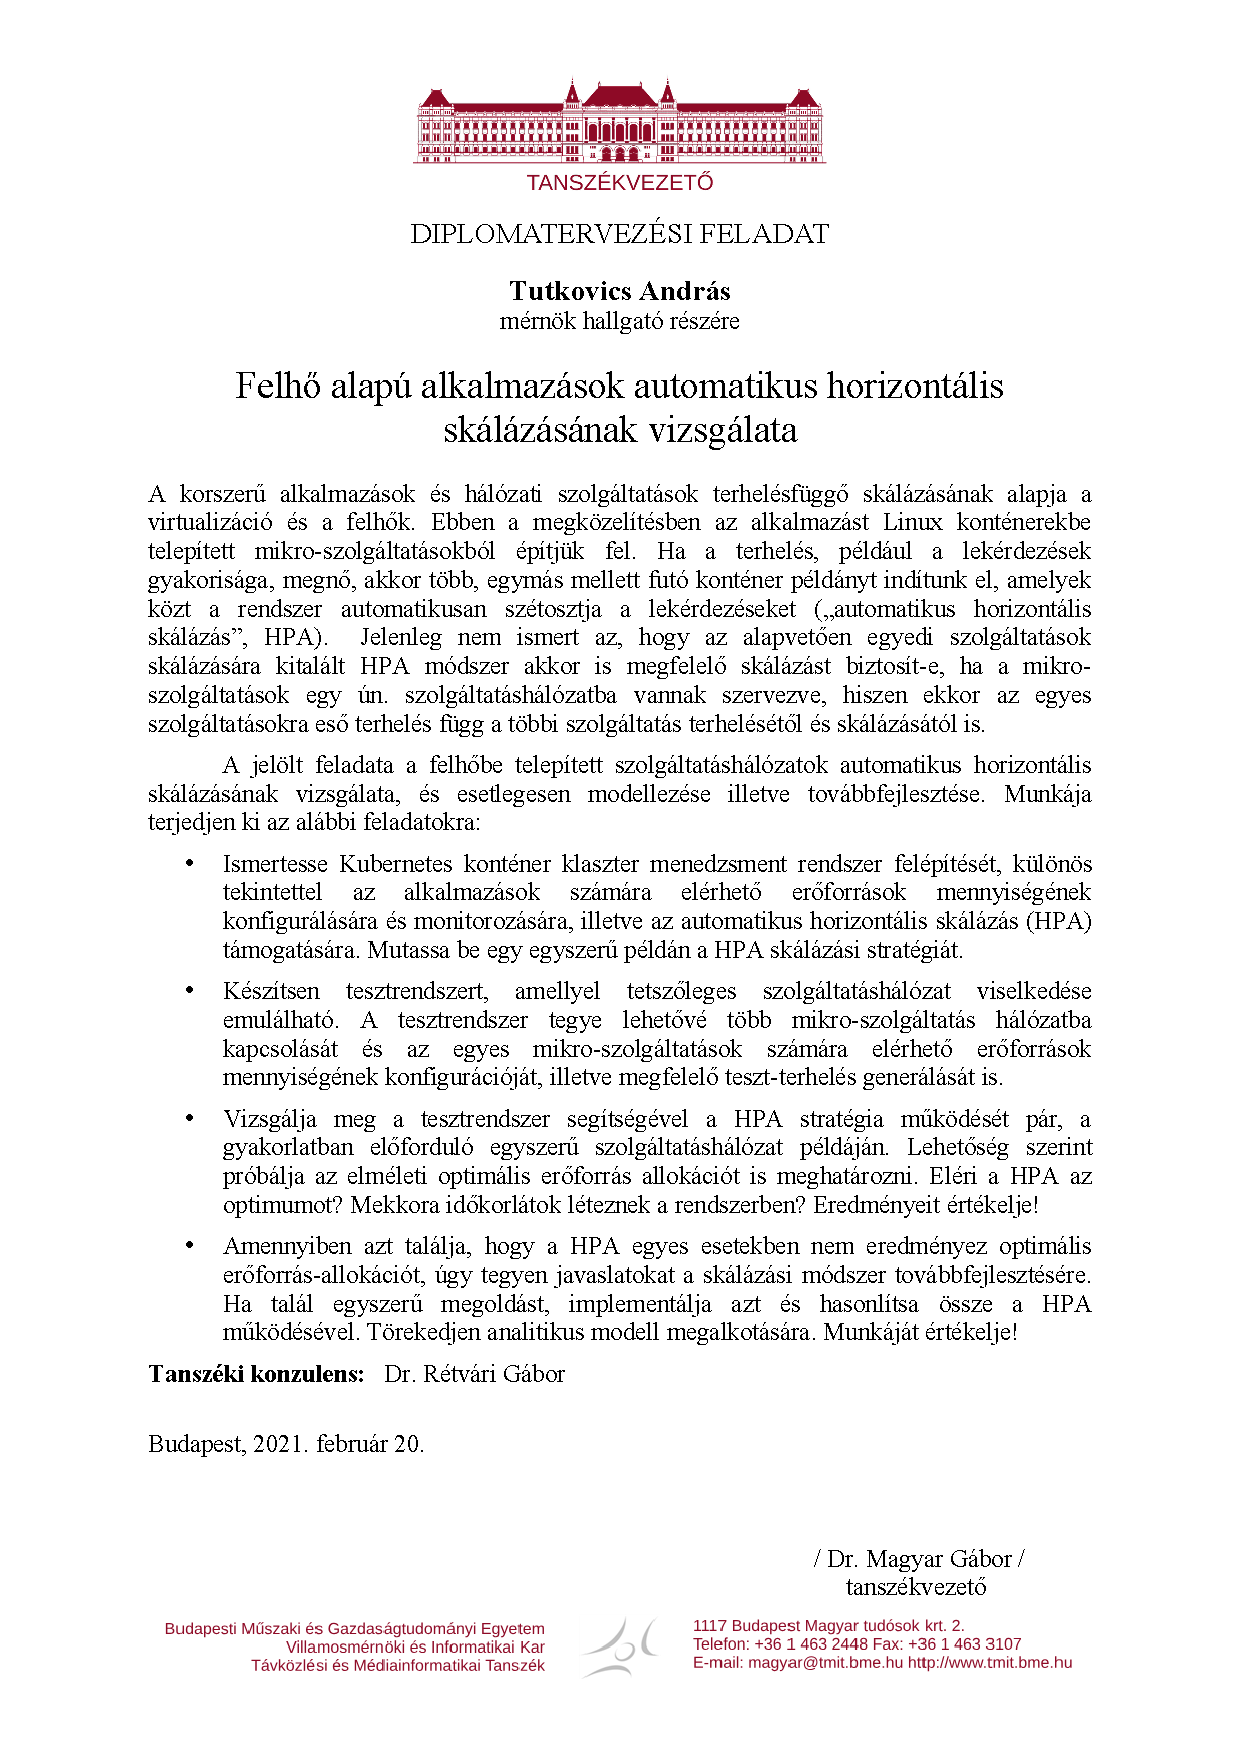
\includepdf[pages=-]{kiiras.pdf}

% Table of Contents
%~~~~~~~~~~~~~~~~~~~~~~~~~~~~~~~~~~~~~~~~~~~~~~~~~~~~~~~~~~~~~~~~~~~~~~~~~~~~~~~~~~~~~~
\setcounter{tocdepth}{2}      % csak a főbb címeket mutassa
\tableofcontents\vfill


% Declaration and Abstract (Diplomatervbe bele kell rakni)
%~~~~~~~~~~~~~~~~~~~~~~~~~~~~~~~~~~~~~~~~~~~~~~~~~~~~~~~~~~~~~~~~~~~~~~~~~~~~~~~~~~~~~~
\selectlanguage{magyar}
\pagenumbering{gobble}
%--------------------------------------------------------------------------------------
% Nyilatkozat
%--------------------------------------------------------------------------------------
\begin{center}
\large
\textbf{HALLGATÓI NYILATKOZAT}\\
\end{center}

Alulírott \emph{\vikszerzoVezeteknev{} \vikszerzoKeresztnev}, szigorló hallgató kijelentem, hogy ezt a \vikmunkatipusat{} meg nem engedett segítség nélkül, saját magam készítettem, csak a megadott forrásokat (szakirodalom, eszközök stb.) használtam fel. Minden olyan részt, melyet szó szerint, vagy azonos értelemben, de átfogalmazva más forrásból átvettem, egyértelműen, a forrás megadásával megjelöltem.

Hozzájárulok, hogy a jelen munkám alapadatait (szerző(k), cím, angol és magyar nyelvű tartalmi kivonat, készítés éve, konzulens(ek) neve) a BME VIK nyilvánosan hozzáférhető elektronikus formában, a munka teljes szövegét pedig az egyetem belső hálózatán keresztül (vagy autentikált felhasználók számára) közzétegye. Kijelentem, hogy a benyújtott munka és annak elektronikus verziója megegyezik. Dékáni engedéllyel titkosított diplomatervek esetén a dolgozat szövege csak 3 év eltelte után válik hozzáférhetővé.

\begin{flushleft}
\vspace*{1cm}
Budapest, \today
\end{flushleft}

\begin{flushright}
 \vspace*{1cm}
 \makebox[7cm]{\rule{6cm}{.4pt}}\\
 \makebox[7cm]{\emph{\vikszerzoVezeteknev{} \vikszerzoKeresztnev}}\\
 \makebox[7cm]{hallgató}
\end{flushright}
\thispagestyle{empty}

\vfill
\clearpage
\thispagestyle{empty} % an empty page

\selectthesislanguage
 % Hallgatói nyilatkozat
\pagenumbering{roman}
\setcounter{page}{1}

\selecthungarian

%----------------------------------------------------------------------------
% Abstract in Hungarian
%----------------------------------------------------------------------------
\chapter*{Kivonat}\addcontentsline{toc}{chapter}{Kivonat}

Jelen dokumentum egy diplomaterv sablon, amely formai keretet ad a BME Villamosmérnöki és Informatikai Karán végző hallgatók által elkészítendő szakdolgozatnak és diplomatervnek. A sablon használata opcionális. Ez a sablon \LaTeX~alapú, a \emph{TeXLive} \TeX-implementációval és a PDF-\LaTeX~fordítóval működőképes.


\vfill
\selectenglish


%----------------------------------------------------------------------------
% Abstract in English
%----------------------------------------------------------------------------
\chapter*{Abstract}\addcontentsline{toc}{chapter}{Abstract}

This document is a \LaTeX-based skeleton for BSc/MSc~theses of students at the Electrical Engineering and Informatics Faculty, Budapest University of Technology and Economics. The usage of this skeleton is optional. It has been tested with the \emph{TeXLive} \TeX~implementation, and it requires the PDF-\LaTeX~compiler.


\vfill
\selectthesislanguage

\newcounter{romanPage}
\setcounter{romanPage}{\value{page}}
\stepcounter{romanPage}    % Magyar és angol nyelvű absztrakt


% The main part of the thesis
%~~~~~~~~~~~~~~~~~~~~~~~~~~~~~~~~~~~~~~~~~~~~~~~~~~~~~~~~~~~~~~~~~~~~~~~~~~~~~~~~~~~~~~
\pagenumbering{arabic}

% Import content
%----------------------------------------------------------------------------
\chapter{\bevezetes}
%----------------------------------------------------------------------------

%----------------------------------------------------------------------------
\section{Motiváció}
%----------------------------------------------------------------------------

Nagyobb távlatból tekintve az informatikai rendszerekre, számos tendenciát figyelhetünk meg a technológia változásával összhangban.
Egy ilyen folyamat, hogy régebben jellemzően dedikált csapat, dedikált nyelven, dedikált alkalmazást, dedikált hardveres erőforrásra fejlesztett éveken keresztül. 
Ennek az eredményei a mostanra megbonthatatlanul nagyra nőtt monolitikus\citep{monoliticAndMicroserviceArchitecture} rendszerek, melyeknek külön szervereket kell biztosítani, hogy azok hiba nélkül tudják kiszolgálni a beérkező igényeket.
Több területen használnak még ilyen rendszereket megbízhatóságuk miatt, ugyanakkor továbbfejlesztésük bonyolult és költséges folyamat.

Anyagi megfontolások mentén beláthatóvá vált, hogy saját fizikai szervereket ilyen szolgáltatások számára nem éri meg fenntartani, mivel azok az idő túlnyomó részében nem használják ki a rendelkezésre álló erőforrásokat.
További faktorokat jelentettek a folyamatosan fejlődő virtualizációs technológiák, melyek lehetővé teszik, hogy a fizikai rendszert absztrahálva, különböző virtuális környezeteket hozzunk létre azok felett.
A megoldásnak köszönhetően lehetőség nyílt előre definiált lépésekkel azonos tulajdonsággal bíró rendszereket létrehozni igény szerint\citep{infrastuctureAsCode}. 
Természetesen mindezt úgy, hogy a fizikailag rendelkezésre álló erőforrások kihasználtsága is javult.

A korábban vázolt monolitikus architektúrát a mai napig sokan alkalmazzák, azonban folyamatos tolódás figyelhető meg a mikro-szolgáltatások irányába, melynek üzleti okai vannak. 
Aki nem tud lépést tartani a gyors fejlődéssel, az rövid időn belül lemarad és hátrányba kerül a versenytársaihoz képest. 
Az érem másik oldala viszont az, hogy aki időben észreveszi a lehetőséget, az hirtelen nagy előnyt tud szerezni. 
Erre jó példa az Amazon\citep{amazon} és a Netflix\citep{netflix} története is.  

Egyre szélesebb körben terjednek el a konténerizációs technológiák és velük együtt az úgynevezett mikro-szolgáltatások\citep{monoliticAndMicroserviceArchitecture}.
A paradigma értelmében a korábbi nagyobb kódegységet szét lehet bontani több kisebb kódbázisra, ami számtalan előnyt jelent az alkalmazás fejlesztésekor.
Mivel a kisebb egységeket könnyebb megérteni mint a teljes kódbázist, az új fejlesztők számára könnyebb becsatlakozni a fejlesztési folyamatokba.
A kisebb elemekre bontott kód lehetőséget biztosít arra is, hogy az egyes komponenseket több nyelven és többfajta keretrendszerben fejlesszük, minden komponens számára az optimális fejlesztési környezetet kiválasztva. 
Végül, ha egy komponens teljes körű felülvizsgálatára van szükség, az nem érinti a rendszer többi részét, amíg a publikus interfészek változatlanok maradnak. 
Ezek által lehetőség nyílik egy kellően agilis rendszer kialakítására, ami könnyebben és gyorsabban tudja kiszolgálni az ügyfelek igényeit, ami üzleti előnyt jelent.

Ez a modern paradigma tartalmaz néhány kihívást is, ami a monolitikus alkalmazások esetében nem merültek fel.
Egy ilyen kihívás kerül tárgyalásra a dolgozatban is.
A tendenciaváltás legnagyobb szereplője a Kubernetes\citep{kubernetesBaseDocumentation}, ami lehetőséget biztosít a konténerizációs technológiák egyszerű és széles körű használatára.

%----------------------------------------------------------------------------
\section{Feladat meghatározása}
%----------------------------------------------------------------------------
A korábban említett paradigmaváltással lépést kell tartani az alkalmazás üzemeltetésekor is. 
Fontos szempont az elkészült, mikro-szolgáltatásokból felépülő hálózat skálázásának kérdése. 
Sokan választották ezt a modern megközelítést, mert ígérete szerint könnyen képes a beérkező kérések okozta terheléssel arányosan skálázódni.
Ez egy triviális feladat egészen addig, amíg az egyes egységeket különálló, másokkal nem összefüggő részként kezeljük.
Ezt megtehetjük és látszólag legtöbben meg is teszik komolyabb fennakadások nélkül, azonban a valóság ennél jóval komplexebb.
Figyelembe kell venni, hogyan kapcsolódnak egymáshoz a mikro-szolgáltatások, azok milyen és mennyi erőforrást használnak, mi történik a beérkező kérésekkel.
A sok szolgáltatás közül melyiket érdemes először skálázni, melyik okozza a kiszolgálások lassulását, milyen módosítással lehet a legtöbb felhasználót kiszolgálni.
Látható, hogy pár paramétert bevéve az egyenletbe a komplexitás meredeken emelkedik. 
Különösen megnehezíti a feladatot, ha a rendelkezésre álló erőforrásokat (például: processzor, memória, hálózat, I/O) globálisan optimálisan szeretnénk elosztani, hogy a lehető legjobb kiszolgálást tudja biztosítani a rendszer. 

A diplomamunka során ezt a kérdéskört kellett megismernem és a felmerülő kérdésekre választ keresni. 
Első lépésben szeretném bemutatni a használt környezetet, a Kubernetes felépítését illetve, hogy milyen skálázási megoldások léteznek és melyiket hogyan támogatja.
Konkrét példán keresztül bemutatom az automatikus pod horizontális skálázó megoldását. 

Egy egyedi keretrendszert kellett összeállítani, ami képes tetszőleges szolgáltatáshálót létrehozni
Kubernetesen belül és azt lekérdezésekkel terhelni. Ezáltal lehetőségünk nyílik szabadon
konfigurálható körülmények között vizsgálni a Kubernetes automatikus horizontális skálázóját, illetve az irodalomban javasolt egyéb megoldásokat is.
Az így nyert eredményekből következtetéseket tudunk tenni az egyes implementációk dinamikáját, költségeit, hatékonyságát illetően.

A feladat része a kapott mérési eredmények vizualizációja is, így könnyebben láthatóvá válnak a
skálázási megoldások és a megoldások közötti különbségek is. 

Az elkészített keretrendszer segítségével, mérési eredményekkel kell bemutatni a Kubernetes felett történő mikroszolgáltatások kommunikációját és figyelni hogyan változik a terhelés függvényében.
Meg kell ismerni, hogy a beépített skálázó működése milyen megoldásokkal jár és milyen helyzetben ad az optimálistól eltérő kiszolgálást.
Ilyen helyzetekre megoldási javaslatokat kell keresni és bemutatni azok működéseit.

%----------------------------------------------------------------------------
\section{A dolgozat felépítése}
%----------------------------------------------------------------------------
A dolgozat fejezetei úgy lettek sorba állítva, hogy azok a lehető legkövethetőbb módon mutassák be a kapott eredményeket. Ehhez viszont az általános részektől kell indulni és így mutatva be az egyre konkrétabb részleteket.
Először szeretném ismertetni a Kubernetes platform architektúráját és az általa támogatott automatikus skálázást \aref{sec:Kubernetes}. fejezetben.
%A \ref{sec:Kubernetes}. fejezetben szó lesz a Kubernetes architektúrájáról, illetve hogyan támogatja beépített módon az automatikus skálázást.
A munka kezdetén el kellett olvasni a témában készült korábbi kutatásokat, amelyeket \aref{sec:Publications}. fejezetben ismertetek.
Ezután \aref{sec:system}. fejezetben bemutatom az elkészített keretrendszert, annak építő elemeit és a megvalósítás során hozott döntéseket. 
Az elvégzett mérések kerülnek ismertetésre \aref{sec:results}. fejezetben, beleértve a kapott eredmények értelmezését is.
A mérési eredmények alapján pár megoldási javaslatot teszek \aref{sec:solutions}. fejezetben, vázolva az előnyeiket és hátrányaikat. 
Végül \aref{sec:summary}. fejezetben összefoglalom a diplomamunkám eredményeit és kitérek az újonnan felmerült kérdésekre, továbbhaladási irányokra.

%----------------------------------------------------------------------------
%\chapter{\Kubernetes}
%\label{sec:Kubernetes}
%----------------------------------------------------------------------------
\chapter{Kubernetes}
\label{sec:Kubernetes}
A diplomamunka keretén belül végzett feladataim jelentős részben támaszkodnak a Kubernetes (K8s) rendszerre, így annak alapvető ismertetése szükségszerű a dolgozat további megértéséhez.
Egy kellően széleskörűen elterjedt platformról van szó, szerteágazó felhasználási területekkel, emiatt a rendszer teljes körű ismertetésére nem vállalkoztam és próbáltam a ténylegesen szükséges információk körére szorítkozni.

%----------------------------------------------------------------------------
\section{Motivációja}
%----------------------------------------------------------------------------
Ahogy egyre többen kezdték megismerni és használni a konténerizációs technikákat, mint például a Docker, úgy egyre tolódott át az üzemeltetési oldal is ilyen irányba. Ezek után nem  az jelentette a kihívást, hogy az egyes alkalmazásokat egy dedikált virtuális gépen kellett beüzemelni és elindítani. Az új igények szerint az alkalmazásunk egyes részeit egymástól függetlenül kellett konténerekben futtatni. Ezáltal sokkal több kisebb részegységre kellett figyelni, ami jelentősen több feladattal jár, mint a korábbi gépek kezelése. 

Ezzel a problémával találkozott a Google is és kezdődött egy platform fejlesztése, ami képes a fenti feladatok megoldására. Eleinte ez a \textit{Borg}\citep{Borg} nevet viselte. Ezt 2014-ben a Google nyílt forráskódúvá tette immáron Kubernetes néven. A projektet a \textit{Cloud Native Computing Foundation (CNCF)}\citep{cncf} vette gondozásába. Innentől kezdve bárki szabadon elérheti és bele is fejleszthet. Az elmúlt 6 év alatt hatalmas fejlődésen ment keresztül és már a $22$.-ik kiadásánál tart.

Egészen fiatal rendszerről van tehát szó, azonban a VMware kutatásából\citep{VMwareSurvey} is sok érdekes dolog bontakozik ki. Egyre többen térnek át a Kubrenetesre és futtatják benne a konténerizált infrastruktúrájukat. Látható, hogy nem egy rövidtávon elmúló trendről van szó és még mindig felívelő ágban van. A kutatásban résztvevők jelentős részére hozott könnyebbségeket főként az erőforrás gazdálkodásban és a fejlesztési ciklusok rövidítésében. Mindössze a megkérdezettek 5\% nem számolt be érezhető előnyről.  

%----------------------------------------------------------------------------
\section{Felépítése}
%----------------------------------------------------------------------------

\subsection{Klaszter elemei}
%----------------------------------------------------------------------------
Kubernetes alatt általában egy teljes klasztert szoktak érteni. Ennek a rendszernek az egyes részeit és azok feladatát szeretném bemutatni.  

\subsubsection{Csomópontok}
A legtöbb klaszter több csomópontot (node) tartalmaz. Ezek lehetnek akár egy egész szerver vagy egy szerveren futtatott virtuális gép is. Itt fognak futni a később részletesen tárgyalt kapszulák, amik az alkalmazásunkat valósítják meg. Ezért itt futniuk kell azoknak a szolgáltatásoknak, amik ezt lehetővé fogják tenni. A csomópontok konfigurációját a vezérlő sík (control plane) végzi. A \ref{k8s_nodes} sorszámmal ellátott kódrészleten láthatjuk, hogy az általunk későbbiekben használt klaszter esetében milyen csomópontok vannak. Fontos, hogy az egyes node nevek  különbözőek legyenek. 

Feladatkörét tekintve két különböző típusú node lehet. Egyik, ami a vezérlő síkot biztosítja, ő az úgynevezett \textit{master} illetve a másik, ahol csak kapszulák futhatnak, ezek a \textit{worker} típusú csomópontok. Látható, hogy a példaként hozott kódrészletben a \verb+dipterv1+ névvel ellátott node van mester szerepben. Az utóbbi időben egyre jobban elmosódott a határvonal a két típus között és több csomóponton van megvalósítva a vezérlő sík, illetve ezeken is lehet kapszulákat futtatni.

\lstset{caption=Később használt klaszter csomópontjai, label=k8s_nodes}
\lstinputlisting{figures/kubectl_get_nodes.sh}

Az egyes csomópontoknak biztosítani kell, hogy futhassanak rajtuk kapszulák. Ezért minden egyes node rendelkezik az alábbi komponsensekkel:

\paragraph{Kubelet} Minden node rendelkezik egy \textit{kublet} nevű ügynökkel (\textit{agent}), mely feladata az adott csomópontra ütemezett konténerek rendszerint futtatása. Ezt úgy tudja megtenni, hogy az API szerveren keresztül kap egy pod leírót és az abban leírtak alapján kezeli a konténereket. Ezen felül feladata, hogy az általa összegyűjtött információkat jelentse a vezérlő sík felé, ezzel lehetővé téve az új konténerek ütemezését csomópontokra. 

\paragraph{Kube-proxy} A \textit{kube-proxy} szintén része minden csomópontnak, ahogy az a \ref{fig:k8s_components} ábrán is látszik. Ezen komponens feladata az adott node hálózatát karban tartani. Ezt úgy tudja megtenni, hogy operációs rendszer szintjén hoz létre és tartja karban a hálózati csomagokra vonatkozó szabályokat.

\paragraph{Konténert futtató környezet} Mivel az egyes kapszulák konténereket tartalmaznak ezért szükség van egy olyan környezetre, ami képes futtatni ezeket a konténereket. Mai napig a legelterjedtebb a Docker, de a Kubernetes ezen kívül még másokat is támogat. 

% Kubernetes cluster components ---------------------------------------------
\begin{figure}[!ht]
\centering
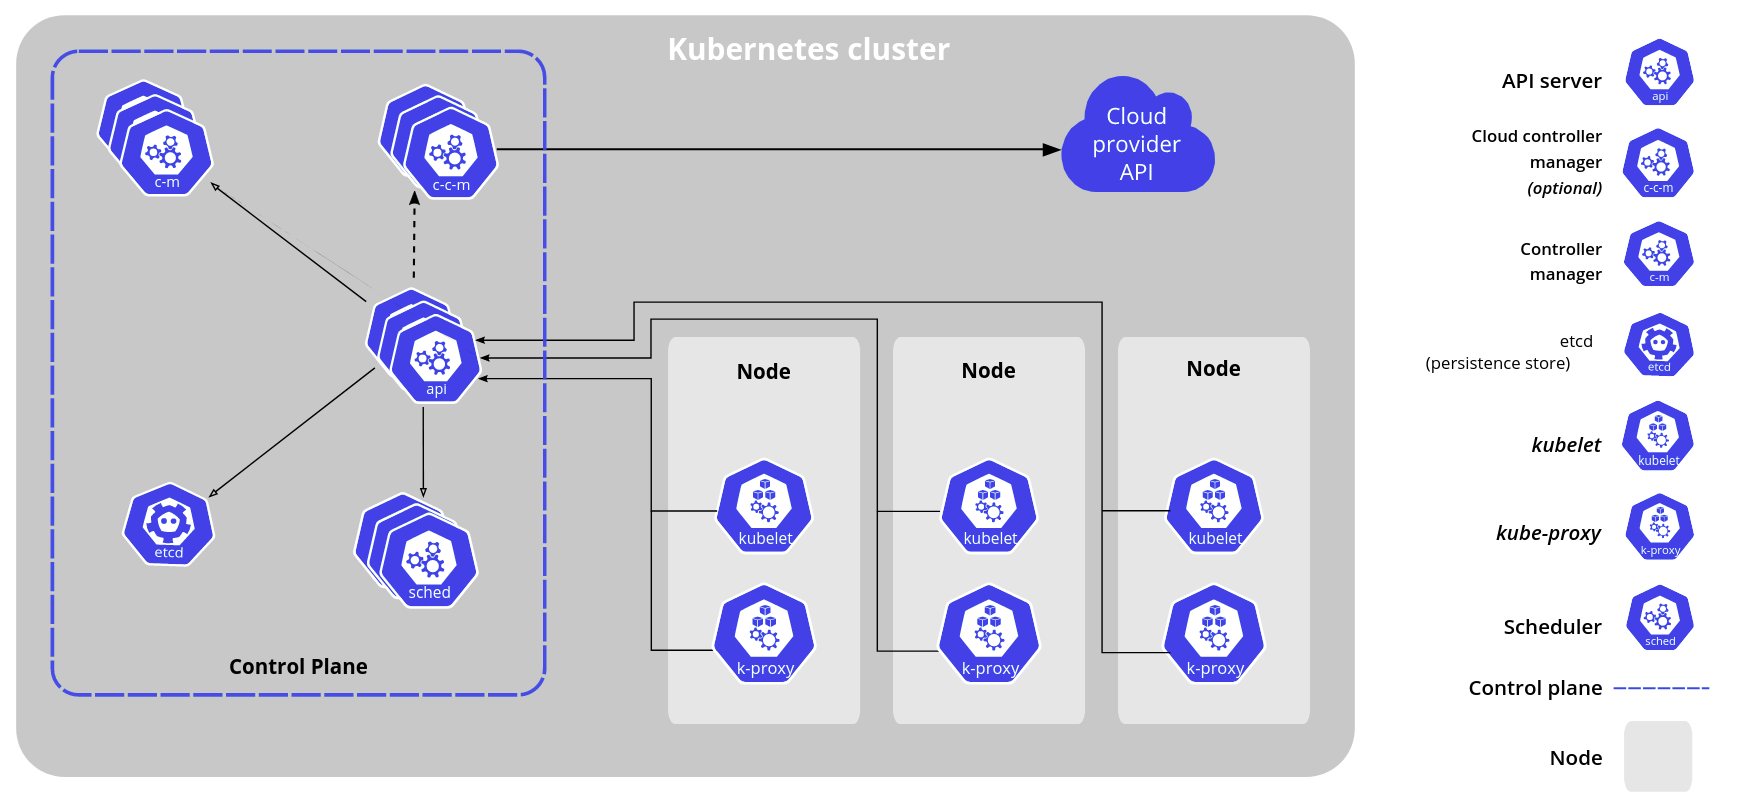
\includegraphics[width=150mm, keepaspectratio]{figures/kubernetes_components.png}
\caption{Kubernetes klaszter elemei\citep{KubernetesComponents}}
\label{fig:k8s_components}
\end{figure}

\subsubsection{Vezérlő sík}
A Kubernetesen belül a vezérlő sík felelős a klaszteren belüli döntésekért. Feladata például meghatározni, hogy az újonnan létrehozandó kapszulák melyik csomóponton induljanak el. A \ref{fig:k8s_components} ábrán is láthatjuk a vezérlő síkot kék szaggatott vonallal keretezve.

\paragraph{API szerver} A klaszter központi egysége. Minden művelet rajta keresztül történik. Ő felelős a beérkező kérések hitelesítéséért és továbbításáért a megfelelő rendszerelemek felé. Például a \verb+kubectl+ parancs használatakor is az történik, hogy a kliensünk összeállít és elküld egy üzenetet az API szerverhez, ami megkapja és válaszol rá.

\paragraph{Etcd} Az \textit{etcd} komponense a vezérlő síknak egy elosztott módon működő\citep{raft} kulcs-érték párokat tartalmazó adatbázis. Itt tárolja a klaszter összes saját tulajdonságát, például az egyes objektumok állapotait is. Ezáltal a korábbi példaként említett \verb+kubectl+ lekérdezésünk is ebből az adatbázisból kiolvasott értékeket fogja megkapni.

\paragraph{Ütemező} Az ütemező (\textit{kube-scheduler}) feladata, meghozni a döntést, hogy egy új pod melyik csomóponton kerüljön létrehozásra. Ez egy igazán izgalmas feladat, hiszen figyelembe kell vennie a rendszer jelenlegi foglaltságát, illetve a kapszula létrehozásakor külön meg lehet adni megkötéseket a node felé. Ilyen megkötés vonatkozhat a csomópont szoftverére vagy hardverére is. 

\subsection{Erőforrások}
%----------------------------------------------------------------------------
Lehetőségünk van a konténerek erőforrás használatához különféle megkötéseket tenni. 
Megadhatunk olyan szabályokat, amik maximalizálják a konténer számára használható erőforrásokat.
Ezen szabályokkal elérhetjük, hogy egy esetlegesen hibásan implementált vagy kártékony alkalmazás a klaszter működésére nagymértékben kihasson az erőforrások mohó használatával.
Másik eset, amikor olyan szabályt adunk meg, ami előre lefoglalja a kellő mennyiségű erőforrást a konténer számára.
Másik jellegű szabályozás, amikor előre lefoglaljuk az alkalmazás által igényelt minimális erőforrásokat.
Kritikus alkalmazások esetében hasznos lehet, mivel ebben az esetben garantálni tudjuk az erőforrások rendelkezésre állását a rendszer többi részétől függetlenül.
Ezeket \verb+request+  és \verb+limit+ értékeknek nevezzük.
Az igényelt erőforrásnál használhat a futó konténer többet is, azonban ez már függ a többi konténertől is.
Limitáció esetén viszont csak a megadott mennyiség állhat a rendelkezésére.
Fontos jól megválasztani az értékét, mert például, ha kevés memóriahasználatot engedélyezünk az egyik konténernek, akkor lehet hogy el sem tud majd indulni és hibát fog jelezni.

Leginkább a processzor- és memóriahasználatra szoktak ilyen megkötéseket létrehozni, de lehetőség
van más erőforrásokat is kezelni.
A konténerek és podok létrehozásakor a \textit{kubelet} ütemezője figyelembe fogja venni a megadott
paramétereket és ez alapján választja ki, hogy melyik csomóponton fog futni. 

\subsection{Objektumok}
%----------------------------------------------------------------------------
A Kubernetes egyik erőssége, hogy az átlagos felhasználás esetében nem kell törődni a rendszer felépítésével, hiszen nekünk csak deklaratív módon meg kell létrehozni és kezelni bizonyos erőforrásokat, objektumokat.
  
\paragraph{Pod (kapszula)}
%\label{par:pod}
A Kubernetesben megjelenő legkisebb logikai egység.
Általában egy konténert futtat, de lehetőségünk van több konténer futtatására is. Általánosságban elmondható, hogy rendszeresen létrejönnek és rendszeresen törölve is lesznek ezek az objektumok, tehát nem tartós életűek.
Ezen tulajdonság miatt a rendszer egészére is célszerű egy dinamikusan változó környezetként tekinteni.

\paragraph{ReplicaSet} 
ReplicaSet felelős az általa kezelt kapszulák számának monitorozásáért. Ennek értelmében, ha az egyik \textit{pod} meghibásodik és megáll, akkor helyette egy újat fog létrehozni. Ezáltal biztosított, hogy mindig a megfelelő számú egység fogja fogadni a beérkező kéréseket és nem kell manuálisan monitorozni a státuszukat.

\paragraph{Deployment}
Mivel \textit{kapszulák} túl kicsi részei a teljes alkalmazásnak és életük sem kiszámítható ezért nem kifizetődő ilyen módon kezelni a rendszerünket. Erre találták ki a \textit{Deploment} objektumot, ahol meg tudjuk adni, hogy milyen \textit{Podok} jöjjenek létre, illetve beállíthatjuk a hozzájuk kapcsolódó \textit{ReplicaSet} értéket is. Ezáltal lehetőségünk van absztrakt szinten deklaratívan módon megadni a kívánt rendszer tulajdonságait.

\paragraph{Service}
A korábban említett objektumokkal már meg tudunk valósítani bizonyos funkciókat, viszont ezt szeretnénk a klaszteren belül és kívülre is elérhetővé tenni. Erre találták ki \textit{Service} objektumot. Ezen keresztül könnyen el tudjuk érni az azonos szolgáltatást nyújtó \textit{kapszulákat} és nem kell az alkalmazás logikában számontartani az ő elérhetőségeiket. Ez ugye különösen nehéz feladat lenne, hiszen a készenléti idejük is elég változó lehet, mivel folyamatosan jönnek létre és törlődnek.

\paragraph{Custom Resources (CR)}
A Kubernetes API lehetőséget biztosít számunkra, hogy tetszőlegesen kibővítsük. Így lehetőségünk van
saját objektumokat is létrehozni, illetve azokat saját kontrollerrel kezelni. Ehhez először egy
saját erőforrás leírót kell létrehozni (Custom Resource Definiton - CRD), ami tartalmazza az
általunk kívánt erőforrás definícióját. Ezzel lehetőséget kapunk, hogy tetszőlegesen komplex
leírásokat hozzunk létre és ezt egy logika deklaratív módon feldolgozza.

%----------------------------------------------------------------------------
\section{Skálázás}
%----------------------------------------------------------------------------
A felhő alapú infrastruktúra egyik legcsábítóbb előnye, hogy az alkalmazásunk képes adaptálódni a külvilág felől érkező kérésekhez. Ez azt jelenti, hogy ha több felhasználót kell egyszerre kiszolgálni, akkor a rendszer automatikusan növeli a kiszolgálásra fordított erőforrások mennyiségét. Ezzel a megoldással elérhetjük, hogy a végfelhasználó ne vegyen észre minőségbeli csökkenést és a kevésbé intenzív időkben pedig nem foglalunk feleslegesen erőforrást, ami az üzemeltetőnek is jól belátható anyagi érdeke.
 
Alapvetően két különböző skálázási módszert lehet elkülöníteni. Az egyik a vertikális, míg a másik a horizontális skálázás. Ezekről a későbbiekben bővebben lesz szó. 

\subsection{Horizontális skálázás}
%----------------------------------------------------------------------------
A két skálázási mód közötti különbséget mutatja a \refstruc{fig:scaling}. Jobb oldalon látható megoldás az úgynevezett horizontális skálázás (másik nevén: scaling out). Ebben az esetben arról van szó, hogy a megnövekedett igények kiszolgálásához több azonos egységet hozunk létre. Az összes egység azonos erőforrás felhasználással rendelkezik és a beérkező kérések köztük lesznek szétosztva. 
A megoldás egyik legnagyobb előnye, hogy elég könnyű alkalmazni, a Kubernetes rendszere is alapértelmezettként támogatja. Hátrányánál meg lehet említeni, hogy több egység között oszlanak meg a beérkező kérések így nem biztos, hogy azonos egységnél köt ki egy felhasználó két különböző kérése. 

\subsubsection{Automatikus horizontális skálázás}
\label{subsec:hpa}
%----------------------------------------------------------------------------
Egy egyszerű példán keresztül szeretném bemutatni a Kubernetes beépített, automatikus horizontális skálázóját (HPA). Az automatikus skálázónak meg lehet adni, hogy milyen célértéket szeretnénk kapni. Például, hogy a futtatott \textit{Pod} által felhasználható CPU mennyiség milyen szinten legyen kihasználva. Jelenleg ilyen megkötést a memória és processzor felhasználásra lehet tenni, de tetszőlegesen létrehozhatunk saját metrikát. 

Az algoritmus folyamatosan lekérdezi a metrikák aktuális értékét és \aref{hpa_algo} egyenlet alapján meghatározza az éppen szükséges replika számot. Ezzel a számított értékkel frissíti a \textit{Pod} replika számát, amit így a replikációért felelős kontroller észlel és megpróbálja elérni a kívánt állapotot. Ezzel módszerrel megvalósítható fel- és leskálázás is.

\begin{equation}
\label{hpa_algo}
desiredReplicas = \left\lceil currentReplicas * \frac{currentMetricValue}{desiredMetricValue} \right\rceil
\end{equation}

A folyamat szemléletesebb, ha konkrét példán nézzük meg működését.
Ehhez először létre kellett hozni egy alkalmazást, amit tudunk majd skálázni.
Ehhez egy egyszerű webszervert használtam, ami minden beérkezett kérés esetén egy CPU intenzív műveletet hajt végre. 
Miután létrejött a szükséges \textit{Deployment} és \textit{Service} utána létre lehetett hozni az automatikus skálázót.
Ennek a forráskódja látható a \ref{hpa_example} kódrészlet tetején.
Be lehet állítani, hogy mi legyen a minimális és maximális replika, ami között lehetősége van skálázni. 
Továbbá definiálni kell egy célértéket is, ami alapján a skálázási döntéseket meg tudja hozni.
A példában látható, hogy $50\%$-os CPU felhasználást szeretnénk elérni.
Fontos, hogy alapvetően a metrikákat a skálázó egy úgynevezett metrika szervertől gyűjti be, amit külön el kell indítani, mert alapértelmezettként nem fut a Kubernetesben.

Ha létrehoztuk a skálázót, ki is lehet próbálni.
Ehhez egy \verb+bash+ szkript segítségével állandó forgalmat generálunk és figyeljük meg, hogyan változik a kapszulák száma és ezzel összefüggően az egyes egységek CPU felhasználása.
Kezdetben $1$ darab \textit{Pod} végezte az összes beérkező kérés kiszolgálását, ami így a célértéknél 3-4-szer több processzort használt.
A korábban mutatott képlet alapján, a felső egész részt vesszük és a jelenlegi replikaszám 4-szeresére skálázunk. \\
 
\lstset{caption=Automatikus horizontális skálázás folyamata, label=hpa_example}
\lstinputlisting{figures/hpa_example.sh}


\subsection{Vertikális skálázás}
%----------------------------------------------------------------------------
A skálázási megoldások közül a másik megoldás a \refstruc{fig:scaling} bal oldalán látható. 
Ezt vertikális skálázásnak (másik nevén: scaling up) hívnak. 
Ebben az esetben a kiszolgáló egységek számát nem módosítjuk, hanem az általuk felhasználható
erőforrások mennyiségét növeljük. Ilyen példa, amikor plusz memóriát rakunk a számítógépbe, vagy
erősebb processzorra cseréljük a meglévőt. Kubernetes jelenleg még nem támogatja alapértelmezettként
ezt a funkciót, de egyszerűen használatra lehet bírni. Előnye a megoldásnak, hogy a korábbi félévek
munkái alatt azt figyeltük meg, hogy a vizsgált alkalmazásaink ezzel a stratégiával azonos erőforrás
felhasználás mellett jobb eredményeket értek el.\citep{bscThesis} Hátránya, hogy a jelenlegi
implementáció szerint a minden skálázásnál le kell állítani a futtatott egységet, ami bizonyos
szolgáltatás esetén nem túl előnyös, hiszen ez idő alatt kevesebb egység végzi a beérkező kérések kiszolgálását.

% Skálázás módjai ábra -------------------------------------------------------
\begin{figure}[!ht]
\centering
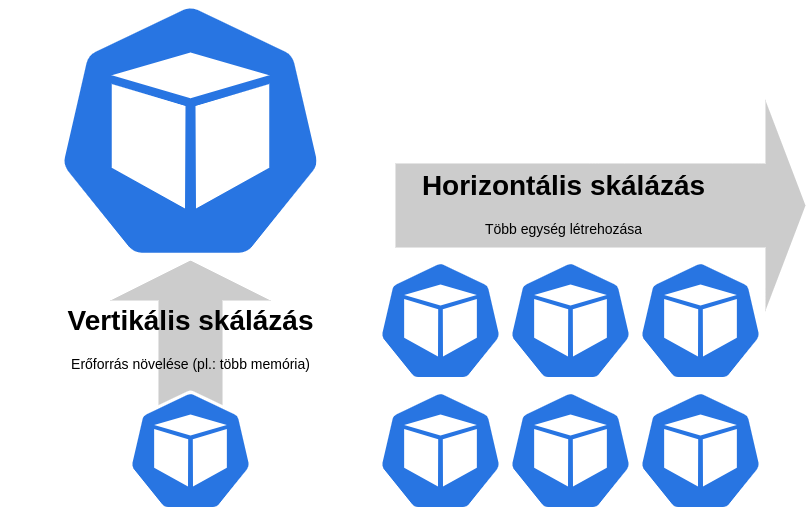
\includegraphics[width=100mm, keepaspectratio]{figures/scaling_types.png}
\caption{Vertikális és horizontális skálázás}
\label{fig:scaling}
\end{figure}

%TODO: VPA leírás kell?

%----------------------------------------------------------------------------
\section{Szolgáltatás minőségi osztályok Kubernetesben}
%----------------------------------------------------------------------------

Következőkben szeretném bemutatni a Kubernetes klaszteren belül megjelenő szolgáltatásminőségi osztályokat, illetve azok működését.
Három különböző minőségi osztály létezik jelenleg a Kubernetes implementációjában\citep{KubernetesQoSClasses}. 
Ezek osztályok ismerete és a kihatásuk az ütemező döntéseire hasznosak lesznek az egyes mérések megtervezéséhez és a kapott eredmények értelmezéséhez.

A Kubernetes minden egyes kapszulához rendel egy minőségi osztályt, amit a beállított erőforrás specifikációkból fog következtetni.
Tehát, csak az egyes podoknak ilyen jellegű attribútumok illetve csak impliciten lehet definiálni.
Az ütemező számára fog hasznos információt nyújtani, amikor dönteni kell az egyes podok csomópontra történő rendelésénél vagy megszüntetéséről.

A kapszulán belüli konkrét osztály meghatározása \aref{get_qos_example} kódrészlet kimenetén látható módon lehet megtenni.
Le lehet kérdezni a \textit{get} és a \textit{describe} paranccsal is, és az előbbit választottam, mert legtöbb esetben bővebb kimenetet kaphatunk, mint a \textit{describe} paranccsal, ugyanis ilyenkor megkapunk minden információt, amit az adott erőforrással kapcsolatban a Kubernetes az \textit{etcd}-ben tárol.

A kimeneten látszik, hogy az érintett erőforrás egy pod, amiben egy darab konténer fut.
A kimenet szükségtelen részét töröltem és csak a számunkra releváns részt hagytam meg.
Látható, hogy egyedül a memória értékre van megkötés, hogy mi legyen a konténer számára maximálisan használható memória mennyiség, ami a példában 170 megabájt. 
Ezzel szemben a pod létrehozásánál létezik megkötés, hogy milyen processzor és memória mennyiségeket szeretne közvetlenül lefoglalni és fixen saját használat alatt tartani.
Könnyen leolvasható, hogy ez a memória esetén 70 megabájt és 100 mCPU processzort jelent.
A számunkra másik fontos részlet már a \textit{status} alatt található.
Itt azok az információk szerepelnek, amiket nem mi definiáltunk és adtunk meg a létrehozás előtt, hanem az erőforrás működése közben változtak.
Többek között ilyenek például, hogy mikor indult el a kapszula, hányszor kellett újraindítani, milyen belső IP címen érhető el illetve a számunka fontos \textit{qosClass} érték is.
Látható, hogy a konkrét példán ez \textit{Burstable} értéket kapott.

\lstset{caption=Adott kapszula minőségosztályának vizsgálata, label=get_qos_example}
\lstinputlisting{figures/burstable-pod.yaml}

A következő alfejezetekben részletesen bemutatom, az egyes osztályok tulajdonságait, és mi alapján lesznek a kapszulák osztályozva.
Láthatjuk, hogy milyen módon van lehetőségünk az egyes alkalmazások között priorizálni, ezt a Kubernetes hogyan fogja kezelni.
Mindezzel együtt érthetővé válik a korábbi példán látott besorolás is.


\section{Garantált minőségű osztály}
%----------------------------------------------------------------------------

A garantált (\textit{quaranteed}) minőségű szolgáltatás osztály élvezi a legtöbb előnyét a Kubernetes ütemezőnek.
Akkor kerülhet ebbe az osztályba egy adott pod, ha több kritériumnak is megfelel.
A kapszulán belül, minden egyes konténerre érvényesnek kell legyenek, az alábbi megkötések. 
Ezek vonatkoznak a rendes alkalmazás konténerre és az init konténerekre is.

\begin{itemize}
    \item Konténeren belül meg van adva az igényelt és maximálisan használható processzor mennyisége.
    \item Konténeren belül meg van adva az igényelt és maximálisan használható memória mennyisége.
    \item Az igényelt erőforrások és a maximálisan használható erőforrások értékei megegyeznek.
\end{itemize}

A fenti kritériumokhoz kapcsolódóan fontos megjegyezni, azt az érdekes esetet, ami akkor áll elő, ha egy konténerhez mindössze az erőforrások limitációját adjuk meg.
Ebben az esetben automatikusan kerül beállításra az igényelt erőforrás értéke, ami megegyezik a limitációval.
Emiatt hiába nem adunk meg expliciten értéket az igényelt erőforrásokhoz, de kitöltjük a limit értékeket, akkor is garantált szolgáltatás osztályba fog kerülni az adott pod.

Ezen kapszulák olyan csomópontokra kerülnek ütemezésre, amik rendelkeznek elegendő erőforrásokkal és a bennük futtatott alkalmazások lesznek a kevés erőforrás miatt utoljára leállítva.

\section{Börsztölhető minőségű osztály}
%----------------------------------------------------------------------------
% ToDo: börsztölhető lehet nem a legjobb kifejezés
A börsztölhető (\textit{burstable}) kapszulák besorolását elég széleskörűen lehet meghatározni.
Leginkább azt lehet mondani, hogy ide tartoznak azok a podok, amik valami miatt nem teljesítik a garantált szolgáltatás osztályba tartozó kritériumokat, azonban valamilyen erőforrás foglalás megvan adva.
Tipikusan ilyen szituáció, amikor különböző értékek vannak megadva az igényelt és a maximálisan használható erőforrások mennyisége között.
Akkor is ide kerül besorolásra egy kapszula, ha több konténer közül valamelyik nem teljesíti a garantált osztály elvárásait.

Ezen podokat igyekszik az ütemező a rendelkezésre álló információi alapján a számukra legjobb csomópontra osztani, de nem garantálható ennek a sikere.
Ez abból fakad, hogy legtöbb esetben kevesebb információval rendelkezik róluk, mint a garantált osztályban, ahol minden érték adott volt.

Amikor elfogynak a csomópont által használható erőforrások és nincsen több legjobb szándék minőségű osztályba tartozó kapszula, akkor ezen podok kerülnek leállításra. 
Ezzel is védve a garantált osztályú podokat.

\section{Legjobb szándék minőségű osztály}
%----------------------------------------------------------------------------
Legalacsonyabb prioritási szinttel a legjobb szándék (\textit{best effort}) minőségi osztály rendelkezik a felsoroltak közül, amire már a neve is utal.
Ide kerülnek az olyan kapszulák, ahol semelyik konténernek nincsen beállítva erőforrásra vonatkozó információ.
Tehát nincs megkötés a maximális használatra és nincs megkötés a minimálisan szükséges erőforrásra se.

Ebben az esetben rendelkezik az ütemező a legkevesebb információval a kapszuláról, ami miatt nem is garantálható, hogy olyan csomóponton kerül elindításra, ahol elegendő erőforrás áll az alkalmazás rendelkezésére.

Ebbe a kategóriába tartozó podok annyi erőforrást használhatnak, amennyi rendelkezésre áll az adott csomóponton.
Emiatt felmerül a veszélye, hogy a többi alkalmazás elől fogja elhasználni a szükséges erőforrásokat. 
Ezzel magyarázható, hogy az osztályba tartozó podok lesznek először leállítva, amikor fogytán van a csomóponton elérhető erőforrások mennyisége.
\\
\\
A fentebb írtak miatt körültekintően kell eljárni az erőforrások szabályozása közben, hiszen ezáltal lehetőségünk van priorizálni az alkalmazásainkat.

%----------------------------------------------------------------------------
%\chapter{\Kubernetes}
%\label{sec:Kubernetes}
%----------------------------------------------------------------------------
\chapter{Irodalomkutatás}
\label{sec:Publications}
A félév során több publikációt is elolvastam, hogy tisztább legyen a kutatási terület. A következőben szeretném összefoglalni, hogy eddig milyen irányban történtek haladások.

Több oldalról meg lehet fogni a skálázás és szorosan hozzá köthető erőforrás elosztás területét. Minden kutatás kicsit más szempontból vizsgálja, más áll a középpontban.

Vannak: reaktív és prediktív modellek.
Prediktív --> ML, MC
  - a nap / hónap / év ciklikusságát használja 
reaktív: fix szabélyrendszer (pl: 50\% kihasználtság felett --> skálázás!)




%----------------------------------------------------------------------------
\chapter{Rendszer felépítése}
\label{sec:system}
%----------------------------------------------------------------------------
Ebben a fejezetben szeretném bemutatni az elkészített rendszert és az azt alkotó egyes elemeket.
A fejezet végén részletezésre kerül egy teljes mérés folyamata és a kapott eredmények feldolgozásának lépései.

%----------------------------------------------------------------------------
\section{Rendszer részei}
%----------------------------------------------------------------------------
Az elkészült rendszer három fő komponensből áll. Ezek együttesen képesek tetszőleges tulajdonsággal rendelkező szolgáltatás hálózatokat megvalósítani, azt Kubernetes alatt elindítani, forgalmat generálni és mérés során adatokat gyűjteni. 

Az egyes részekről bővebben is lesz szó, azonban most átfogóan ismertetem a rendszert, ami a \ref{fig:system_overview} ábrán látható. Minden elem megalkotásánál egy lényeges szempont volt, hogy az elkészült rendszerrel könnyen lehessen méréseket indítani és a lehető legtöbb paraméter konfigurálható legyen.

A mérések paramétereit egy konfigurációs fájlban tudjuk megadni, ahonnan egy Python program olvassa be és vezényli le a mérések elvégzését.
Először a Kubernetes API-n keresztül létrehoz egy \textit{ServiceGraph} objektumot, ami nem egy beépített típus.
Az objektum értelmezéséhez és megfelelő kezeléséhez létre kellett hozni egy operátort, ami képes egy ilyen definíció szerint létrehozni a szükséges erőforrásokat (\textit{deployment, pod, service, HPA}).

Ahhoz, hogy az egyes kiszolgáló egységeket is tudjuk tetszés szerint konfigurálni kell egy olyan képfájl, ami a megadott paraméterek alapján tud működni.
Ezért írni kellett egy külön alkalmazást hozzá.

Miután elkészültek a kért objektumok és képesek már kiszolgálni a klaszteren kívülről érkező igényeket a Python szkript elkezd számukra forgalmat generálni.
A terhelés lejárta után ki kell nyerni a mérés során keletkezett adatokat.
A feladat elvégzésében segítségünkre lesz a Prometheus\citep{Prometheus} alkalmazás, ami gyűjti és exportálja a klaszterből érkező metrikákat. 

Az elkészült rendszerhez szükséges részek forráskódjai megtalálhatóak a GitHub felületén\citep{gitRepo}. 

% Rendszer áttekintése -------------------------------------------------------
\begin{figure}[!ht]
\centering
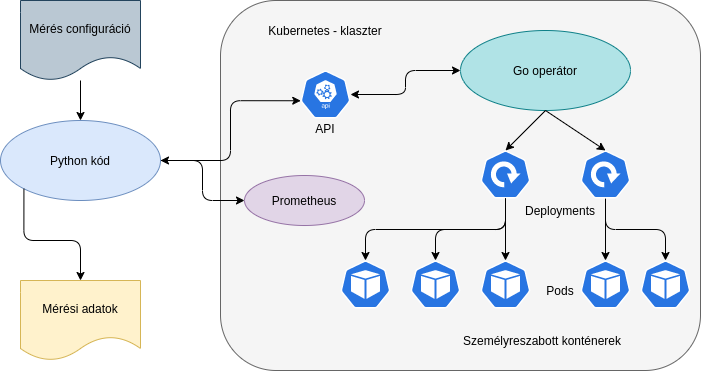
\includegraphics[width=150mm, keepaspectratio]{figures/system_overview.png}
\caption{Rendszer áttekintése}
\label{fig:system_overview}
\end{figure}

%----------------------------------------------------------------------------
\section{Korábbi munkák}
%----------------------------------------------------------------------------
A korábbi projekttárgyak keretén belül már foglalkoztam hasonló kérdéskörrel, így már volt az egyes eszközök használatához tapasztalat és implementáció is, amiből ki lehetett indulni. 
Önálló labor tárgyban megismerkedtem a Go programozási nyelvvel, és elkészítettem egy Kubernetes operátort, ami képes egyedi erőforrás definíciók feldolgozására és ez alapján képes beépített objektumokat létrehozni. A félév elején elején ezt tovább kellett bővíteni, hogy képes legyen skálázót is létrehozni valamint javítani kellett a megbízhatóságán is.

Korábbi tanulmányaim során elkezdtem készíteni egy Go nyelven íródott alkalmazást, aminek a célja azonos volt a mostani projektben foglalttal.
A megkezdett alkalmazás is egy kellően szabadon konfigurálható paraméterezéssel rendelkező webszerver volt, hogy tetszőleges módon tudja kiszolgálni a beérkező kéréseket. 
A korábbi állományból elindulva kellett fejleszteni a funkcionalitásán, hogy valósághűbb eredményeket tudjon szolgáltatni.

%----------------------------------------------------------------------------
\section{Operátor}
%----------------------------------------------------------------------------
Fontos szempontnak tekintettük, hogy egyszerű konfigurációs fájl alapján létre lehessen hozni a szolgáltatáshálót, amit szeretnénk tesztelni.
A Kubernetes rendszer nem tartalmaz olyan erőforrást, ami számunkra ezt a funkcionalitást alapvetően támogatná.
A feladat számunkra az lesz, hogy egy közös konfiguráció alapján több különböző fajta, már beépített erőforrást hozzunk létre.
Már az orkesztrációs platform fejlesztésénél felkészültek arra az esetre, hogy sok egyedi igény fog megjelenni a különböző használatból fakadóan, ezért már fejlesztés közben fontos szempont volt a Kubernetes könnyű kibővítése.
A mögöttes gondolat az, hogy nagyon változó igények és funkcionalitások jelenhetnek meg a felhasználási körülményektől függően, amiket nem célszerű a központi egységbe implementálni, hiszen akkor a rendszer könnyen átláthatatlanná és inkonzisztensé válna.
Helyette egyedi erőforrásokat (CustomResource) hozhatunk létre és ezen erőforrások mellé megadhatunk különböző vezérlőket. Ezt csinálják az operátorok, amivel a fentebb vázolt feladat a diplomamunkában is megoldhatóvá vált.

\subsection{Megírása}
%----------------------------------------------------------------------------
A klaszter operátorral való kibővítése egy gyakran alkalmazott megoldás, amikor összetettebb alkalmazást vagy logikát kell implementálni.
Olyan szinten elterjedt megoldásról van szó, hogy több nyelv és keretrendszer közül lehet választani\citep{availableOperatorFrameworks}.
Létezik továbbá egy külön weboldal a korábban megírt és publikált operátorok böngészésére, ami kiindulási pontként szolgálhat a forráskódok tanulmányozására.\citep{operatorhub} 
A Kubernetes alkalmazási lehetőségei között ezt a megoldást külön mintaként említik.\citep{KubernetesPatterns} 

Én a feladat megoldásához az Operator-SDK\citep{operatorSDK} keretrendszerét használtam fel. 
A keretrendszerrel könnyen írhatunk Kubernetes operátorokat.
Ezt megtehetjük Helm, Ansible vagy Go segítségével is.
A felsorolt opciók közül a Go programozási nyelv adja a legnagyobb rugalmasságot, mivel lehetőségünk van nagyon mély szinten belenyúlni a klaszter működébe.
Én is ezt a megoldást választottam a korábbi projekttárgy keretén belül és sikerült megszerezni az alapvető ismerteket. 
Feladatom volt a korábban megírt alkalmazás hibáinak javítása és új funkciókkal történő bővítése.

Sajnos limitált számú segédanyag érhető el és azok is többnyire ugyanazt a példaalkalmazást mutatják be, ezért az elején nehéz belekezdeni. Egyedül a korábban mások által megírt operátorok forráskódja tudott jó kiindulásként szolgálni.

Több megoldás is létezik az elkészült operátorunk futtatására. Futtathatjuk a klaszteren kívülről, mint alkalmazást, illetve a klaszteren belülről is. Utóbbi esetben készíteni kell az alkalmazásunkból egy Docker képfájlt, ami aztán külön kapszulában fog futni. Illetve klaszteren belül lehetőségünk van egy úgynevezett operátor életciklus kezelővel (Operator Lifecycle Manager - OLM) is megtenni ezt. Az utóbbi megoldás a legfejlettebb úgy kell elképzelni mint egy külön csomagkezelő csak a klaszteren belül, az operátoroknak. A félévben én a klaszteren kívüli megoldást használtam, mivel az operátort is folyamatosan fejleszteni kellett a különböző igények szerint, illetve a projekt kapcsán nem releváns az operátor futási környezete, cserébe több idő marad a mérésekre koncentrálni.

\subsection{Használata}
%----------------------------------------------------------------------------
A \ref{servicegraph_example} kódrészlet mutat egy példát a szolgáltatásháló definíciójára. Számunkra elég végiggondolni, hogy milyen szolgáltatásokat szeretnénk, hogyan kövessék egymást, milyen erőforrást biztosítsunk számukra. Miután ezek megvannak készítünk belőle egy \textit{yaml} dokumentumot.

Látható, hogy a \verb+apiVersion+ és \verb+kind+ érték egyedi, így tudunk hivatkozni a saját erőforrásunkra. Szintén meg kell adni pár meta információt, mint például az objektum neve és névtere. A \verb+spec+ szekció az érdekes számunkra. Itt tudjuk felsorolni, hogy milyen szolgáltatásokat szeretnénk majd a hálózatba. Be tudjuk állítani, hogy hány replikával fusson egy-egy szolgáltatás, illetve hogy milyen portokon tudjuk majd őket elérni. Ezek az információk azért lesznek fontosak, mert ez alapján fog az operátor létrehozni Kubernetes Deploymenteket és Serviceket. Ha szeretnénk skálázást is beállítani az adott szolgáltatásra akkor azt is megtehetjük, ha megadjuk a \verb+hpa+ konfigurációs paramétereket. Ezek hiányában nem kerül létrehozásra, és fix replikaszámmal fog üzemelni.

Továbbá definiálni kell, hogy az adott szolgáltatás milyen végpontok hívására figyeljen. Például a \textit{front-end} szolgáltatás a \verb+/instant+ és \verb+/chain+ lekérdezésekre fog válaszolni. A válasz gyorsasága és a közben felhasznált erőforrás mennyiséget is lehetőségünk van befolyásolni. Az itt megadott paraméterek továbbításra kerülnek majd a futtatott konténerekhez így ők fogják helyileg érvényre juttatni a szabályokat. 

A bemutatott kód csak részlete a teljes forrásállománynak, mert elég repetitív ezért nem szerettem volna a helyet foglalni, de a GitHub oldalán megtalálható a teljes kód. \\

\lstset{caption=Saját szolgáltatásháló definiálása, label=servicegraph_example}
\lstinputlisting{figures/servicegraph.yaml}

A szolgáltatásháló definíciójának leírása után, annak kezelése nem jelent gondot.
Az új erőforrás Kubernetesben történő regisztrációja után a futó operátorunk már képes értelmezni a megadott leírót.
Ezáltal felhasználói oldalról egy beépített típusnak megfelelően tudjuk kezelni a saját \verb+Servicegraph+ objektumunkat is.
Egy példa indítás látható \aref{servicegraph_apply} kódrészletben, amikor a \textit{kubectl} parancson keresztül meghívjuk a Kubernetes API-t és továbbítjuk a hivatkozott konfigurációs fájlban leírtakat számára.
Innen kerül feldolgozásra az operátor által, ami létrehozza a kívánt erőforrásokat a klaszteren belül. 
A második sorban láthatjuk a visszaküldött üzenetet, miszerint sikeresen létrejött az új objektumunk.

\lstset{caption=Szolgáltatásháló indítása, label=servicegraph_apply}
\begin{lstlisting}[language=bash,morekeywords={kubectl, apply},alsoletter={-},breaklines=true]
$ kubectl apply -f path/to/servicegraph.yaml                          
servicegraph.dipterv.my.domain/servicegraph created 
\end{lstlisting}


%----------------------------------------------------------------------------
\section{Alkalmazás konténer készítése}
%----------------------------------------------------------------------------
A korábban látott módon lehetőségünk van tetszőleges szolgáltatásokat elindítani, azonban hogy az adott szolgáltatásoknak további paraméterek tudjunk átadni, olyan alkalmazás kell ami tudja kezelni őket. Például: milyen végpontokra figyeljenek, milyen kiszolgálási idővel dolgozzanak, mennyi erőforrást használjanak fel.
A feladat megoldására létrehoztam egy Go alapú webalkalmazást, mely induláskor átveszi a szükséges paramétereket. A webszerverhez beérkező kérések pedig a megadott paraméterek által specifikált módon fognak végrehajtódni. 

A teljes kódbázis részletes ismertetése túlmutatna a dolgozat keretein, ezért ettől szeretnék eltekinteni.
A mérések során használt kódok és a Docker képfájl készítéséhez szükséges minden forrás, erőforrás és instrukció megtalálható a diplomamunkához tartozó verziókövető rendszerben\citep{gitRepo}. 
Azonban szeretném kiemelni a számomra izgalmasnak ítélt részeket és említésre méltó megoldásokat.

Az alkalmazás elkészítéséhez fel tudtam használni a korábbi egyetemi tárgyak alatt elkészített forráskódot, melynek továbbfejlesztése szükséges feladat volt.
A korábbi verzióban \textit{html} alapú válaszüzenetet kaptunk vissza az alkalmazástól, ami megjelenítve számunkra könnyebben áttekinthető, azonban automatizáláshoz nehezen használható.
Így módosítani kellett a kódot, hogy a visszaadott üzenet \textit{json} alapú legyen, ezzel segítve az eredmények későbbi feldolgozását.

Lehetőségünk van a \textit{http} kérés kiszolgálása közben további webalkalmazások felé lekérdezéseket indítani.
Ez a funkció lehetőséget ad, hogy a klaszteren belül tetszőleges szolgáltatáshálókat valósítsunk meg, azonban fejleszteni kellett rajta.
Lecseréltem ezen lekérdezéseket aszinkron hívásokra, hogy a válaszra várakozás közben elvégezhetővé váljon a saját csomópontban szükséges számítások végrehajtása. 

\subsection{Processzor-használat skálázása}
%----------------------------------------------------------------------------
Egyik legfontosabb feladata az egyes podokban elindított alkalmazásnak, hogy fel tudja dolgozni a számára átadott paramétereket.
Kintről kell átadni minden olyan értéket, ami meghatározza a működési módját.
Többek között meg lehet adni, hogy az egyes végpontokra érkező kérések esetén mekkora processzor igényt generáljon.
Ezen funkció implementálása bizonyult a legérdekesebb feladatnak.

Az alkalmazás első funkcióiban nem kapott még jelentős figyelmet, mert a nagy rendszer összeállítása került fókuszba.
Emiatt egy egyszerű processzor igényes algoritmust implementáltam, ami a feladatát tökéletesen ellátta.
Az általam választott algoritmus az Eratoszthenész szitája volt, ami képes megkeresni egy bizonyos számig létező prímszámokat.
Az algoritmusban szereplő lépések nem nehezek, azonban több egymásba ágyazott \textit{for} ciklust tartalmaz, ami így beláthatatlan ideig de használja a rendelkezésre álló processzort.
További érdekesség, hogy amikor a végeredményt nem került kiírásra vagy felhasználásra, akkor a fordító valószínűleg figyelmen kívül hagyta a számára feleslegesnek hitt műveletsort és nem került bele a végleges alkalmazásba.
Ez a tulajdonsága a fordítónak egyszerre barátságos, mert már fordítás közben is javítja a kódminőséget azonban egyszerre kiszámíthatatlanná teszi a kész programunkat, mert hiába írtuk meg nem került meghívásra a függvény.

A megoldás gyengeségét az adta, hogy nem lehet finomhangolni és a Kubernetesben létező mCPU mértékegység szerint konfigurálni az alkalmazás egységünket.
Amikor a rendszer fejlesztésének előrehaladott szakaszában ez a probléma ismét előkerült, megoldási javaslatot kellett keresni.

A megoldás alapját az úgynevezett szoros ciklusok (\textit{tight loop}\citep{tightLoop}) adta.

A mögöttes elgondolás, hogy 1000 mCPU felhasználást akkor kapunk, ha a megfigyelt konténer egy teljes másodpercig birtokolja és ezen idő alatt folyamatosan használja is az erőforrást.
Viszont előre meghatározni, nem lehet, hogy mennyi műveletet végezzünk, hiszen ezt befolyásolja a Kubernetes klaszter mögötti infrastruktúra.
Tehát elképzelhető, hogy azonos algoritmus futása eltérő terhelésként jelenik meg az adott rendszerben értelmezett 1 CPU egység miatt.

A fenti következménye, hogy ha a Kubernetes mCPU mértékegységét akarjuk használni, akkor kötelező lesz az alkalmazás tényleges működése előtt egy kalibrációs tesztet végezni.

Az alkalmazás indításakor futtatott függvényében egy másodpercig egy egyszerű tight loop algoritmust futtat és figyeljük, hogy ezen idő alatt hány iterációt tud megtenni.
Amennyiben az ez információ adott könnyen tudunk generálni megadott terhelést bármilyen környezetben.
Ehhez az kell, hogy a beérkező kérés esetén a korábban kiszámolt iterációk számához arányosan az igényelt processzor-fogyasztással megegyező iterációt tegyen meg. 

A végeredményül előállt megoldás által lehetőségünk van finomhangolni és kontrollálni az egyes lekérdezések hatására keletkező processzor terhelést és annak idejét is. 

\subsection{Elkészült alkalmazás használata}
%----------------------------------------------------------------------------
Az elkészült alkalmazást fel kellett készíteni, hogy a Kubernetesben tudjuk futtatni. Ehhez Docker képfájlt készítettem belőle és miután elláttam a megfelelő címkékkel feltöltöttem\citep{dockerContainer} a Docker Hub oldalra, ami egy ingyenes és publikus konténer adattár. \\

\lstset{caption=Konténer futtatása és válasza, label=describe_pod}
\lstinputlisting{figures/describe_pod.sh}

A \ref{describe_pod} sorszámú kódrészleten egy, az elkészült Docker konténert futtató kapszula leírásának részlete látszik. Az indításhoz a korábban látott, \ref{servicegraph_example} kódrészlet konfigurációját használtam fel. Érdemes megfigyelni, hogy az egyes  paraméterek hogyan képződnek le a konténerhez. Például átadásra kerül a szolgáltatás neve, hogy melyik porton fog figyelni, melyik végpontok hívására kell válaszolnia és a hozzá tartozó egyéb paraméterek.

A kódrészleten látott második paranccsal létrehozunk egy újabb kapszulát a klaszterben. Látható, hogy interaktív módban indítottuk el, így kaptunk egy felületet, ahonnan lekérdezést lehet indítani a \textit{front-end} kapszula felé. Ez jó megoldás abban az esetben, ha ki szeretnénk próbálni, hogyan működik az alkalmazásunk. A \verb+kubectl run+ parancs alatt látható, hogy a \textit{curl} alkalmazás kérésére milyen választ kaptunk. A válasz \textit{json} formátumban tartalmazza a lekérdezés főbb paramétereit. Látható, hogy melyik végpontra érkezett, milyen konfiguráció van beállítva a végponthoz.



%----------------------------------------------------------------------------
\section{Mérés vezénylése}
\label{sec:measure_orchestrate}
%----------------------------------------------------------------------------
Az elkészített operátorral és konténerizált alkalmazásunkkal tetszőleges szolgáltatáshálót képesek vagyunk létrehozni.
A következő megoldandó kihívás a mérések kezelése volt, mivel törekedtem a precíz eredményekre. 
Fontos szempont volt, hogy a mérések elvégzése a lehető legegyszerűbben és rugalmas módon tudjon megtörténni. 
A feladat megvalósításához a Python nyelvet választottam, hiszen könnyen lehet benne szkripteket fejleszteni illetve komoly számítást nem fog végezni így nem számottevő a plusz erőforrás-felhasználása, más alacsonyabb szintű nyelvekhez képest sem. 

Mérés megkezdése előtt készíteni kell egy konfigurációs fájlt. Erre egy példa látható a \ref{measurement_config} kódrészleten. A mérést vezénylő alkalmazás az itt megadott paraméterek alapján fogja végezni a mérést. Többek között meg kell adni, hogy a mérések milyen szolgáltatáshálózatokon kerüljenek elvégzésre. Lehetőség van többet is megadni, így egy indítással akár az összes számunkra érdekes esetet le tudjuk szimulálni egyszerre. Továbbá meg kell adni, hogy milyen kérés per másodperc (\textit{QPS}) értékekre vagyunk kíváncsiak. Fontos megadni, hogy milyen forgalmat és hova szeretnénk generálni. Ez látható a \verb+Load+ részen belül. Megadjuk a mérés idejét, IP címet és portot, ahol a szolgáltatásunk fogja fogadni a kéréseket.\\


\lstset{caption=Mérés konfigurációja, label=measurement_config}
\lstinputlisting{figures/measurement_config.yaml}

A forgalom generálását egy külön alkalmazás végzi, a \textit{Vegeta}\citep{vegetaGithub}. 
Természetesen többféle forgalom generáló alkalmazás használata is lehetséges és a rendszer fejlesztése közben kettőt is kipróbáltam.
A korábbi döntés a \textit{Fortio} generátorra esett, mert könnyen használható, egyre szélesebb körben elterjedt, Go nyelven íródott és ideális döntésnek tűnt a méréseinkhez.
Azonban a folyamatos mérések közben számos  nehezen értelmezhető jelenséget produkált, ezért került sor a váltásra. 

Számos alkalmazást megnéztem, hogy minél körültekintőbb döntést tudjak hozni. 
Ebben nagy segítségemre volt egy összegyűjtött alkalmazás lista\citep{benchmarkToolsList}, így nem kellett megkeresni az egyes eszközöket, hanem csak össze kellett hasonlítani és kipróbálni azokat.
Végül a döntés a \textit{Vegetára} esett, mert hasonló funkcionalitásokkal rendelkezik, mint a korábbi eszközünk, ami jelentősen megkönnyítette a komponens cseréjét.

Egy-egy terhelés szimulációjához meg kell adnunk pár paramétert az alkalmazás indításához. 
%Egy valódi indítást mutat be a  \ref{vegeta_command} kódrészlet. 
Ilyen például az elérni kívánt QPS érték, a terhelés időtartama, a megcélzott végpont, az eredmények mentési neve és helye.
Ezeket a paramétereket a korábban ismertetett konfigurációs fájl alapján állítjuk elő. \\

%\lstset{caption=Példa a \textit{Vegeta} indítására, label=vegeta_command}
%\lstinputlisting[language=Bash]{figures/vegeta_command.sh}

Miután megterheltük a rendszert és megkaptuk a kérések kiszolgálásával kapcsolatos statisztikákat a \textit{Vegetából}, szükséges még a rendszer erőforrás-felhasználását célzó metrikákat is begyűjteni. 
Erre a \verb+Prometheus+ rendszerén keresztül van lehetőségünk.
A szoftver támogatja az API hívásokat, így lehetőségünk nyílik könnyen lekérdezni az általa gyűjtött statisztikákat. 

A metrikák lekérdezésére a \ref{prometheus_query} kódrészlet ad egy példát. Meg kell adnunk, hogy milyen értékekre vagyunk kíváncsiak. A látható példában ez a konténerek által felhasznált CPU mennyisége, továbbá kikötéseket teszünk, hogy csak a \textit{Default} vagy \textit{Metrics} névtérben futó konténerek érdekelnek.
Meg kell adni a lekérdezés kezdeti és vég idejét, amíg a generált kéréseket kiszolgálta.
Össze kell állítani a \verb+Prometheus+ elérhetőségét, amihez a mérés elején megadott konfigurációt vesszük alapul. Ha megvan az előkészített API hívás, akkor a kódrészletben látott módon meg kell hívni azt. A kapott választ \verb+json+ formátumban érkezik, így később mi is így kezeljük. \\


\lstset{caption=\textit{Prometheus} rendszer használata Python kódból, label=prometheus_query}
\lstinputlisting{figures/prometheus.py}

A korábban látott megoldással egyéb adatokat is metrikákat is lekérdezhetünk. Jelenleg négy értéket gyűjtünk:
\begin{itemize}
  \item Konténerek processzor felhasználásait külön-külön.
  \item Konténerek memória felhasználásait külön-külön.
  \item Az összes futó \textit{Pod}, ami részt vesz a mérésben.
  \item A futó konténerek száma típus szerint. (például: külön amik a front-end szolgáltatást valósítják meg és külön amik a back-end szolgáltatást)
\end{itemize}

A \verb+Prometheus+ egészen kiterjeszthető rendszer így közel tetszőleges metrikákat lehet gyűjteni. 


A mérés végén miután összegyűjtöttük az összes keletkező adatokat, beleértve a \verb+Prometheus+ és \verb+Vegeta+ rendszereket is és az eredeti konfigurációt is azokat perzisztálni kell. Erre a legkézenfekvőbb módszer az adatok kiírása \verb+json+ fájlba. Ez azért is előnyös, mert könnyen olvasható és feldolgozható a formátum. 

%----------------------------------------------------------------------------
\section{Eredmények ábrázolása}
%----------------------------------------------------------------------------
Az egyes mérések kimenetei \textit{json} fájlok, melyek értelmezése és ezáltal a következtetések levonása számunkra nehéz feladat lenne ebben a formában. 
Szükségessé vált tehát egy külön alkalmazás implementálása, ami az általunk kapott eredményeket könnyen átlátható formában ábrázolja. 

A feladat megoldására szintén a Python nyelvet választottam, mert könnyen lehet benne fájlokat kezelni, egyes objektumokat módosítani és rendelkezik grafikus megjelenítő modullal.
Fontos szempont volt az alkalmazás könnyű használata ezért bizonyos paramétereket akár parancssorban, indításkor is meg lehet adni. 
Ezáltal az alkalmazás működését tudjuk befolyásolni a konkrét forráskód módosítása nélkül.
%Indításnál megadhatjuk, hogy milyen nevet szeretnénk a grafikonnak, milyen címke legyen az $X$ és $Y$ tengelyeken, hogy le akarjuk-e menteni az ábrát, illetve a legfontosabb, hogy melyik mappában keresse a mérési eredményeket. Egy példa konfiguráció is látható a korábban hivatkozott kódrészlet alján. \\

% Rajzoló program indítása --------------------------------------------------
%\lstset{caption=Eredményeket feldolgozó alkalmazás használata, label=python_drawer}
%\lstinputlisting{figures/python-drawer.sh}

Az alkalmazás indításakor meg kell adni, hogy hova vannak mentve a mérések során készült kimeneti \textit{json} fájlok, melyek feldolgozása szükséges.
Itt egy-egy mérés a forgalomgenerátor által, adott terhelés mellett, adott ideig történő szimulációját értjük.
Ebből következik, hogy egy teszteset futtatása több ilyen értelemben vett mérést tartalmaz, hiszen egy skálán megy végig a rendszer, ahol a minimális QPS értéktől megadott lépésközzel halad a maximális QPS értékig. 
Egyesével elkezdi beolvasni a mérési eredményeket és minden fájlból készít egy "tisztázott" eredményt.
Ebben már csak az adott grafikon kirajzolásához nélkülözhetetlen értékeket tartalmazza.
Például előfordul, hogy a Prometheus eredményében szerepel olyan pod is, ami nem vett részt az adott mérésben, mert még a korábbiból maradt ott.
Az ilyen eseteket észlelni kell és kiszűrni az értékeit, hogy ne okozzanak anomáliákat. 

%----------------------------------------------------------------------------
\section{A mérés és az eredmények feldolgozásának elemei}
\label{sec:measure_steps}
%----------------------------------------------------------------------------

A következő alfejezetben szeretném a korábban bemutatott alkotóelemeket egymás utáni sorba tenni és az általuk végrehajtott egy-egy lépést részletesebben bemutatni.
A fő célja, hogy egy szimulációt teljes egészében bemutasson a mérés indításától kezdődően a kapott eredmények feldolgozásáig.

A bemutatott lépések az elkészült rendszer működésének használatára koncentrálnak, emiatt a Kubernetes operátor működése nem szerepel fajsúlyos mértékben a leírtak között.
Az operátor működését ebben az esetben tekintsük egy beépített szolgáltatásnak.

A lépések könnyebb követhetőségét segíti \aref{fig:measurement_and_draw_workflow} ábra.
A mérés elindításához szükségünk van egy konfigurációs állományra, amiben a kívánt szimulációhoz szükséges paraméterek kerültek definiálásra.
Ebben a konfigurációs fájlban kell megadni azt vagy azokat a szolgáltatáshálót leíró \textit{ServiceGraph} erőforrás \textit{yaml} fájlokat, amiken a szimulációkat futtatni szeretnénk.
Több ilyen szolgáltatás háló is megadható, ebben az esetben többször fog lefutni a szimulációnk azonos paraméterekkel.

Az elindított Python alkalmazás először ellenőrzi, hogy létezik-e parancssorban megadott konfigurációs állomány.
Amennyiben nem volt megadva, a program futása közben is lehetőségünk van azt behivatkozni, ráadásul ebben egy automatikus kiegészítő funkciói is segítségünkre van.
Ha ez megtörtént, akkor egy segédmodul segítségével beolvassuk a paramétereket és eltároljuk egy Python szótárba, hogy később könnyebb legyen az adott értéket felhasználni.

Ezután minden, megadott szolgáltatásháló esetén el kell végezni a következő terheléseket.
Először ki kell számolni, hogy milyen QPS értékű terheléseket fog generálni.
Ha van még ilyen ilyen QPS érték, amire nem lett elvégezve a terhelés, akkor megigényli az éppen aktuálisan vizsgált szolgáltatáshálót a Kubernetes klaszterben.
Ez alapján az operátor elkezdi létrehozni a szükséges erőforrásokat. 
Eközben az alkalmazásunk folyamatosan figyelemmel követi, hogy az igényelt kapszulák állapota futó legyen, hiszen csak a rendszer teljes elindulása után lehet a méréseket elkezdeni.

Miután elindultak a podok bizonyos előmelegítést végez a rendszer, ha a konfigurációs fájl alapján szükséges.
Ez a funkció akkor lehet hasznos, ha nem szeretnénk rögtön a friss rendszeren méréseket végezni, hanem adunk neki egy kis időt és terhelést, hogy felvegyen egy alapállapotot.
Ebben az esetben viszont figyelni kell arra, hogy a Prometheusban megjelenő adatok nem valósidejűek és ez befolyásolhatja a mért eredményeket.
Emiatt a dolgozatban bemutatott méréseknél ezzel a lehetőséggel nem éltem.
A funkció hiba nélküli alkalmazásához további fejlesztések szükségesek.

Az előmelegítési fázis után következhet a valódi terhelés generálása.
Ehhez jelenleg a parancssoros alkalmazást, a Vegetát használom.
Miután a konfigurációban beállított ideig a megadott QPS értékkel történő terhelés befejeződött, szükséges egy kicsit várni.
Erre amiatt van szükség, hogy a Prometheushoz is megérkezzenek a mérés során generált statisztikák.

A mesterséges késleltetés után le kell futtatni az egyes Prometheus lekérdezéseket.
Itt megaddható, hogy milyen felbontással, mettől-meddig és milyen értékeket kérdezzen le.
A rendszerből érkező egyes \textit{json} válaszokat össze kell fűzni, illetve a mérő eszköz által generált statisztikákat is érdemes kezelni.

A különböző forrásokból összeállított kimeneteket egy nagy fájlba kell kimenteni, hogy a későbbiekben is fel tudjuk azokat használni.
A fájl mentése után törölhető a szolgáltatás háló, hogy a következő QPS értékkel történő mérésnél ne zavarjon be a korábbi rendszer és az azon végzett  mérések, így a lehető legtisztább eredményeket kapjuk.
Tehát ezt minden terhelési értékre és szolgáltatási hálón végig kell járni és az egyes kimeneti eredményeket letárolni.

Eddig tart a mérést vezénylő Python alkalmazás hatásköre és feladata.
Amikor előálltak a kimenetek, akkor készen állnak a további feldolgozásra, azonban ezt már egy következő alkalmazás fogja végezni.
Ezért is szerepel más színnel \aref{fig:measurement_and_draw_workflow} ábrán, ahogy azt a bal alsó sarokban található jelmagyarázat is tartalmazza.

Az ábrázolás folyamata a korábban bemutatott lépésekhez képest lineárisabb, emiatt könnyebben is értelmezhető.
Az ábrázoló szkript indításakor szintén bizonyos paraméterek megadása kötelező, hiszen meg kell adni, hogy melyik mappában szereplő mérési eredményeket szeretnénk grafikonra vinni.
A megadott mappában található és értelmezhető \textit{json} típusú fájlokat fogja az alkalmazás egymás után beolvasni.

A beolvasott fájl igazán nagyméretű és rendezetlen adathalmazt tartalmaz.
Emiatt szükséges a nyers adatokat tisztítani és csak a számunkra értelmezhető információkat megtartani.
Az így kapott adatokat transzformálni kell, hogy a későbbiekben az alkalmazás könnyebben tudja ábrázolni.

Az kinyert és előkészített adatokat el kell tárolni, amíg minden mérési eredményt tartalmazó fájlon megtörténik ez a lépés. 
Ennek a folyamatnak a végére előállnak az ábrázolható adatok együttese.
Ezeket különböző módon tudjuk ábrázolni és megjeleníteni.
A kész grafikonokat lehetőségünk van lementeni, de ez csak egy opcionális lépés, emiatt szerepel az ábrán szaggatott vonalas nyíllal.
A megjelenített ablak bezárása után végére is értünk a folyamatnak.

% Mérés lépései -------------------------------------------------------------
\begin{figure}[!ht]
\centering
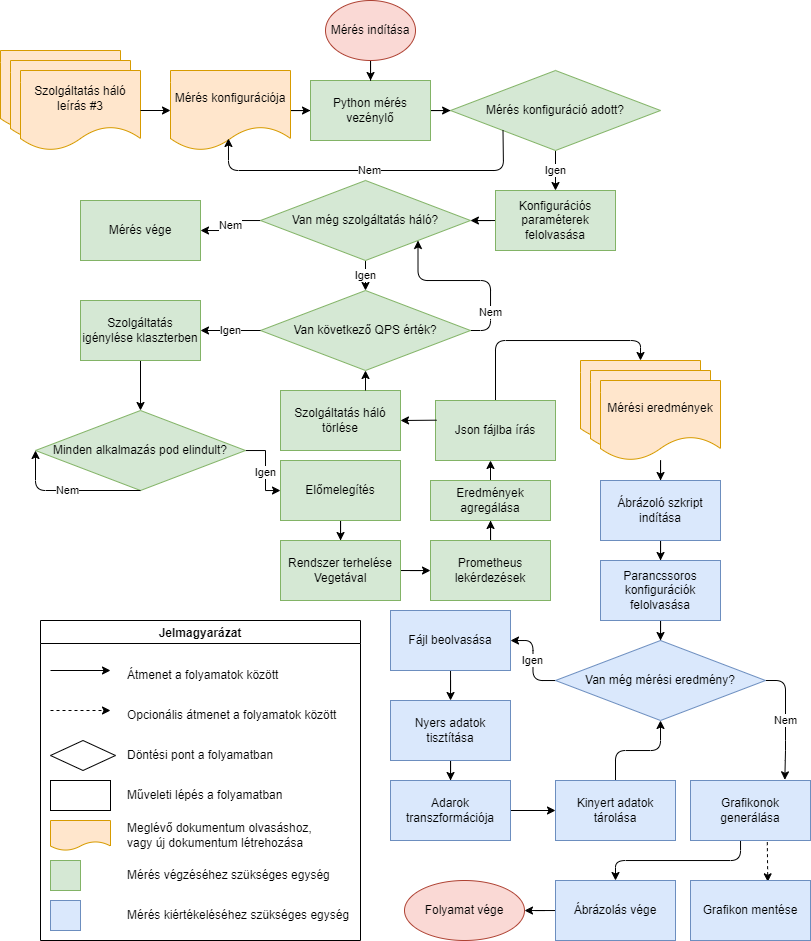
\includegraphics[width=150mm, keepaspectratio]{figures/measurement_and_draw_workflow.png}
\caption{Szimuláció futtatásának és kiértékelésének lépései}
\label{fig:measurement_and_draw_workflow}
\end{figure}


%----------------------------------------------------------------------------
\chapter{Mérések}
\label{sec:results}
%----------------------------------------------------------------------------

A következő fejezetben szeretném bemutatni, hol és hogyan készültek a mérési eredmények, azokból mi olvasható ki. Fontos megjegyezni, hogy komolyabb mérések még a diplomamunka hátralevő részére vannak ütemezve, az alább bemutatott eredmények a rendszer működőképességét igazolják és némi előretekintést nyújtanak.

%----------------------------------------------------------------------------
\section{Mérés környezete}
%----------------------------------------------------------------------------
A feladat elején főként implementációval kellett foglalkozni így nem kapott jelentős szerepet a Kubernetes klaszter. Ezért  a félév első felében elég volt lokálisan futtatni, amit én Minikube (v1.17.1) segítségével tettem meg. 

Amikor a fejlesztési rész kezdett véglegesedni kellett egy rendes környezet, a rendes mérésekhez. Ehhez több lehetőséget is számításba vettem.	

\begin{itemize}
  \item \textbf{BME Cloud}: Egyik lehetőség az egyetemi felhő volt. Itt létre lehet hozni virtuális gépeket, amiket aztán klaszterbe lehet szervezni. Hátránya viszont, hogy hosszabb távra nehezen lehet gépet igényelni, rendszeresen le is állítják ami könnyen okozhatja egy-egy mérés elvesztését, hiszen több órán keresztül is futhat.
  \item \textbf{Klaszter a felhőben}: Kézenfekvő megoldás lehet igényelni egy teljes, egész klasztert. Erre több opció is van, csak hogy a legnagyobbakat említsem: Google, Amazon, Microsoft. Ezek a minőségi szolgáltatások azonban havidíjasok lennének, és bizonyos tekintetben kevésbé rugalmasak. TODO: készültek becslések a havidíjra.
    \item \textbf{Tanszéki infrastruktúra}: A tanszéken létezik egy előretelepített klaszter, amin lehetne méréseket készíteni, de általában foglalt.
      \item \textbf{VM igénylés a Schönherz kollégiumtól}: A Villamosmérnöki és Informatikai Karhoz tartozó Schönherz kollégiumban lévő Kollégiumi Számítástechnikai Körtől lehet tanulmányokhoz és egyéb projekthez kapcsolódóan virtuális gépeket igényelni. Az igénylés leadása után lehetőséget kaptam három virtuális gép használatára egészen a projektfeladat végéig. Bizonyos hátulütőkkel ezen lehetőségnél is számításba kellett venni. Ilyen például, hogy öntevékeny körként hiba esetén a többinél lassabb válaszidőkre lehet számítani.
\end{itemize}		

A fenti opciók közül számomra a negyedik volt a legszimpatikusabb így kaptam is három teljesen új virtuális gépet. Telepítéshez a Debian (v10 - Buster) operációs rendszert választottam, mert stabil, megbízható és széles körben támogatott. A virtuális gépek tulajdonságai az \ref{tab:nodes} ábrán láthatóak. Hasonló erőforrásértékekkel rendelkeznek, annyi különbséggel, hogy csak az egyik gépnek van publikus címe. Továbbá a táblázat tartalmazza az egyes csomópontok nevét és a klaszteren belüli szerepét is.

\begin{table}[ht]
\centering
  \begin{tabular}{c|cccc}
	  Tulajdonság & VM 1 & VM 2 & VM 3 \\
    \hline
	CPU (mag) & 4 & 4 & 4 \\ 
	Memória (GB) & 4 & 4 & 4 \\
	Tárhely (GB) & 10 & 10 & 10 \\  
	Node neve & dipterv1 & dipterv2 & dipterv3 \\ 
	Külső IP & 152.66.211.2 & $\varnothing$ & $\varnothing$ \\ 
	Belső IP & 10.151.103.1 & 10.151.103.2 & 10.151.103.3 \\
	K8s szerep& control-plane,master & worker & worker \\
  \end{tabular}
  
  \caption{Használt csomópontok tulajdonságai}
\label{tab:nodes}
\end{table}

\subsection{Klaszter előkészítése}
%----------------------------------------------------------------------------
A virtuális gépekből klasztert kellett szervezni, amire különböző megoldások léteznek.\citep{kubernetesInstall} Két különbözőt szeretnék kiemelni:
\begin{enumerate}
  \item \textbf{Kubespray}: \textit{Ansible} felhasználásával előre definiált lépéseket hajt végre. Mindössze egy pár soros konfigurációt kell írni hozzá és ígérete szerint minden mást elintéz.
  \item \textbf{Kubeadm}: Az előzőhöz képest a \textit{kubeadm} jóval manuálisabb módszer. Segítségével le tudunk generálni mindenféle kulcsot a klaszterhez, csomópontokat bekötni a rendszerbe.
\end{enumerate}

Nem szándékosan de kipróbáltam mindkét megoldást. Vonzó volt ugyanis a Kubespray, hogy könnyen és automatikusan telepít minden függőséget. Sajnos pont amiatt mert ilyen magas szinten vezeti a telepítést hiba esetén nem sok információ derült ki. Miután eredménytelenül zárult minden próbálkozás, újratelepítettem a virtuális gépeket és áttértem a Kubeadm használatára. 

A telepítés menetét nem részletezném, mert a hivatalos weboldalon látható lépéseken kellett végigmenni. Az elkészült klaszter egy mester csomópontot és kettő kiszolgáló csomóponttal rendelkezik. A fő csomópont rendelkezik egyedül külső hálózatról elérhető, publikus IP címmel, a többinek csak belső címen érhetőek el. Ez némiképpen nehezítette a telepítés folyamatát, részben emiatt sem működött a Kubespray megoldása. 

A klaszter elkészülte után még pár függőséget ki kellett elégíteni, hogy a lokálisan összeállított mérő keretrendszer működni tudjon. Külön telepíteni kellett egy konténer hálózati interfészt (CNI). Ez alapból nem jön a Kubernetessel így külön kell installálni, hogy a különböző csomóponton futtatott konténerek tudjanak egymással kommunikálni. A választás a \textit{Cilium} szoftverre esett, mert szerettem volna jobban megismerni, széleskörűen használható és jól dokumentált. Telepítése után lehetőségünk van teszteseteket futtatni, ami igazolja a klaszterben a csomópontok és kapszulák kommunikációját. 

A \ref{sec:measure_orchestrate} szakaszban leírt módon a mérések során gyűjtött adatok jelentős részét a Prometheus rendszere gyűjti össze és tőle kérdezzük le. Emiatt az éles méréseket végző klaszterben is telepíteni kellett. Ebben a Helm, Kuberneteshez készített csomagkezelő megoldása segített. A \verb+prometheus-stack+ csomagot kellett telepíteni annyi kiegészítéssel, hogy kintről is elérhetővé tegyük a felületet és szolgáltatásait. Azt úgy érhetjük el, hogy a létrehozandó \verb+Service+  típusát \verb+NodePort+-ra állítjuk és a következetesség miatt adunk neki egy portszámot. Az így létrehozott környezet rendelkezik egy webes felhasználói felülettel is, ahol tetszőleges lekérdezéseket indíthatunk. Egy ilyen lekérdezés látszik az \ref{fig:prometheus_example} ábrán is. A példán az látszik, hogy milyen eredményt kapunk, ha lekérdezzük az aktuálisan futó kapszulákat a \verb+Default+ és \verb+Metrics+ névtérben. Az eredményből leolvasható, hogy jelenleg 3 darab \textit{back-end}, 2 darab \textit{front-end} és 1 darab \textit{db} névvel ellátott konténer fut. \\

% Prometheus példa -------------------------------------------------------
\begin{figure}[!ht]
\centering
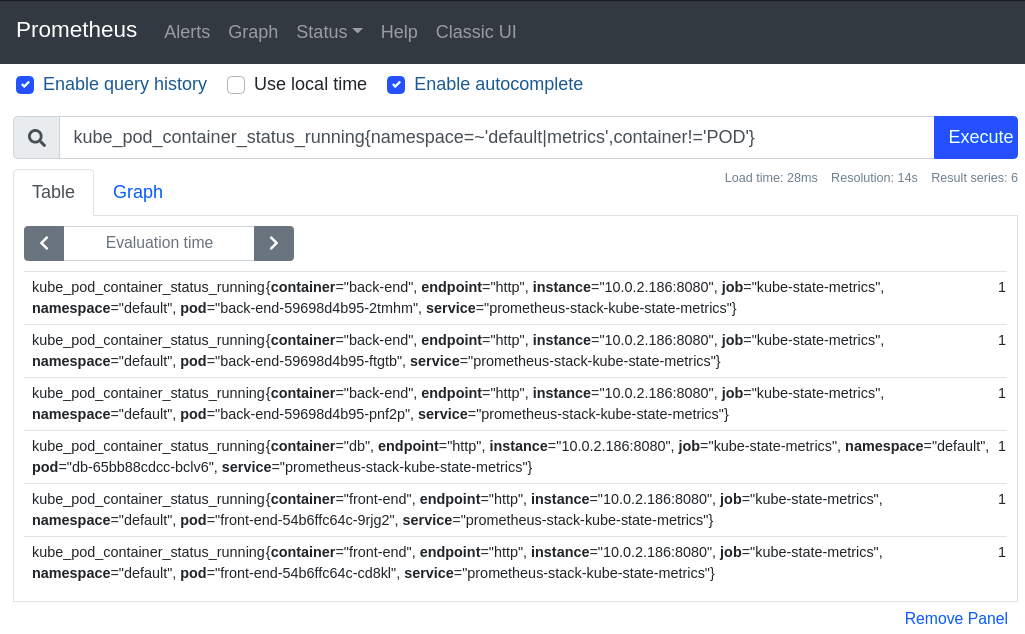
\includegraphics[width=150mm, keepaspectratio]{figures/prometheus_example.png}
\caption{Telepített \textit{Prometheus} rendszere}
\label{fig:prometheus_example}
\end{figure}

Az aktuális rendszerben az operátor még nem külön konténerként fut egy kapszulában, hanem a klaszteren kívül, lokálisan a szerveren, mint egy Go alkalmazás. Emiatt külön telepíteni kellett a Go nyelvet is, hogy el tudjon indulni a rendszer.

\subsection{Verziók}
%----------------------------------------------------------------------------
A rendszer és mérések összeállításához sok különböző komponenset kellett integrálni. Az \ref{tab:versions} táblázat összefoglalóan tartalmazza az egyes környezetek és használt eszközök verzióit. 

\begin{table}[ht]
\centering
  \begin{tabular}{l l}
	  Szoftver 		& Verzió \\
    \hline
      Go 			& 1.16.3 \\ 
      Kubernetes 	& 1.21.0 \\ 
      Kubectl 		& 1.21.0 \\
      Cilium 		& 1.9.5 \\
      Python 		& 3.7.3 \\ 
      Prometheus 	& 2.24.0 \\ 
      Grafana 		& 7.5.3 \\ 
      Operator-SDK 	& 1.4.0-32 \\ 
      Debian 		& 10 (buster)  \\ 
      Istio			& 1.11.4 \\
  \end{tabular}
  
  \caption{Használt verziók}
\label{tab:versions}
\end{table}


%----------------------------------------------------------------------------
\section{Eredmények kiértékelése}
%----------------------------------------------------------------------------
Az egyes méréseknek a kimenete egy-egy \textit{json} fájl, azonban ebből nem nagyon tudunk használható következtetéseket kiolvasni. Szükségessé vált egy külön alkalmazás implementálása, ami az általunk elkészített mérések eredményét fel tudja dolgozni. 

A feladat megoldására szintén a Python nyelvet választottam, mert könnyen lehet benne a \textit{json} objektumokat beolvasni és feldolgozni.
Fontos szempont volt, hogy minél könnyebben használható legyen az alkalmazás, így bizonyos paramétereket akár parancssorban is meg lehet adni. Ez látható az \ref{python_drawer} kódrészleten. Indításnál megadhatjuk, hogy milyen nevet szeretnénk a grafikonnak, milyen címke legyen az $X$ és $Y$ tengelyeken, hogy le akarjuk-e menteni az ábrát, illetve a legfontosabb, hogy melyik mappában keresse a mérési eredményeket. Egy példa konfiguráció is látható a korábban hivatkozott kódrészlet alján. \\

% Rajzoló program indítása --------------------------------------------------
\lstset{caption=Eredményeket feldolgozó alkalmazás használata, label=python_drawer}
\lstinputlisting{figures/python-drawer.sh}

Az alkalmazás indításakor meg kell adni, hogy hova vannak mentve a korábbi mérések során készült kimeneti fájlok. Itt egy-egy mérés jelentése, hogy a Fortio adott darabszámú lekérdezést generál másodpercenként fix ideig. Tehát egy teszteset futtatása több ilyen értelemben vett mérést tartalmaz, hiszen egy skálán megy végig a rendszer, ahol a minimális QPS értéktől megadott lépésközzel halad a maximális QPS értékig. 
Egyesével elkezdi beolvasni a mérési eredményeket és minden fájlból készít egy "tisztázott" eredményt. Ebben már csak az adott grafikon kirajzolásához nélkülözhetetlen értékeket tartalmazza. Például előfordul, hogy a Prometheus eredményében szerepel olyan pod is, ami nem vett részt az adott mérésben, mert még a korábbiból maradt ott. Az ilyen eseteket észlelni kell és kiszedni az értékeit, ne okozzanak anomáliákat. 

%----------------------------------------------------------------------------
\section{Példa mérés}
%----------------------------------------------------------------------------
A rendszer összeállítása után méréseket is lehet már végezni. A mérés mérésben két szolgáltatás vett rész, ahogy az az \ref{fig:sample_sg} sorszámú ábrán is látszik. A szolgáltatáshálóban két különböző feladatot ellátó szolgáltatás szerepelt. Volt egy nodeport segítségével kintről elérhető \textit{front-end} szolgáltatás, illetve egy csak bentről elérhető \textit{back-end}. Azt a szituációt vizsgáltuk, amikor a \textit{front-end} nem használ sok erőforrást, és két pod fut belőle. Ezzel szemben a \textit{back-end} egy jóval erőforrásabb szolgáltatás, cserébe három egység fut belőle. A \textit{front-end} minden felé érkező, \verb+/to-backend+ végpontra érkező kérést továbbított a \textit{back-end} \verb+heavy+ végpontjára. Ezzel elértük, hogy a második szolgáltatásunk a számára beállított, sok processzort igénylő műveletet hajtsa végre.


% Példa szolgáltatás háló----------------------------------------------------
\begin{figure}[!ht]
\centering
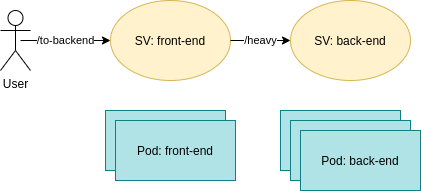
\includegraphics[width=100mm, keepaspectratio]{figures/sample_measurement.png}
\caption{A mérésnek kitett szolgáltatások kapcsolata}
\label{fig:sample_sg}
\end{figure}

A kapott eredményekből készült grafikon látható az \ref{fig:example_plot} és \ref{fig:example_responsetime} ábrán. 

A kapott \ref{fig:example_responsetime} ábráról leolvasható, hogy az átlagos válaszidő a mérés során nem változott érdemben, végig kellően alacsony maradt. Fontos megjegyezni, hogy a mérés során nem vittünk a rendszerbe mesterséges késleltetést, csak a kötelező műveletek elvégzését vártuk meg, így jött ki az állandó válaszidő.

A másik, \ref{fig:example_plot} grafikonon látható, hogy a kevésbé erőforrás-igényes \textit{front-end} processzor felhasználása lassan de folyamatosan nő egészen addig, amíg a \textit{back-end} is tudja növelni a processzor felhasználását. Ez körülbelül 125 QPS-ig tart. Ilyenkor a \textit{back-end} eléri az indításkor beállított erőforrás limitációt és emiatt nem tud több beérkező igényt kiszolgálni.  Emiatt a felhasználói forgalmat generáló Fortio sem fog tudni több kérést a rendszer felé küldeni, mert meg kell várja, mire a \textit{front-end} válaszol, de a front-end csak azután válaszol, hogy meghívta a végletekig megterhelt \textit{back-end} szolgáltatást.

Érdemes figyelembe venni, hogy az $X$ tengely az igényelt lekérdezések darabszámát mutatja, nem a rendszer által valóságban kiszolgált kérések mennyiségét. \\


% Generált példa ábrák -------------------------------------------------------
\begin{figure}[!ht]
\centering
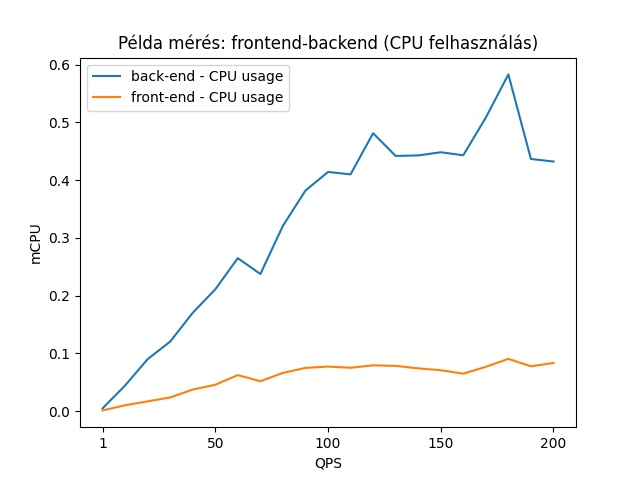
\includegraphics[width=150mm, keepaspectratio]{figures/sample_plot_cpu.jpg}
\caption{\textit{Front-end} és \textit{back-end} egységből álló rendszer CPU felhasználása}
\label{fig:example_plot}
\end{figure}

\begin{figure}[!ht]
\centering
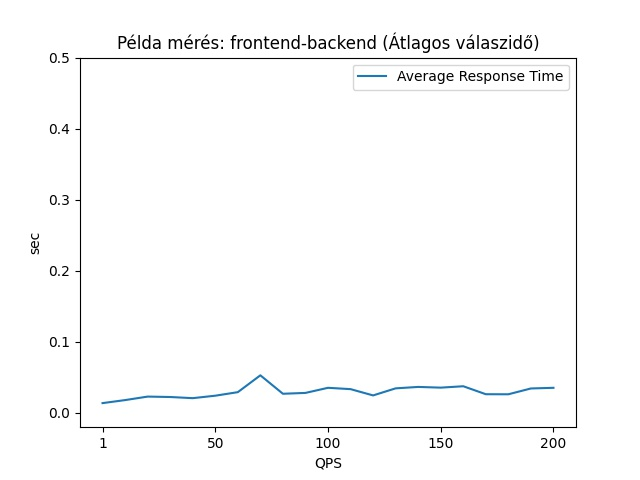
\includegraphics[width=150mm, keepaspectratio]{figures/sample_plot_responsetime.jpg}
\caption{\textit{Front-end} és \textit{back-end} egységből álló rendszer átlagos válaszideje}
\label{fig:example_responsetime}
\end{figure}


%----------------------------------------------------------------------------
\section{Finomhangolás}
%----------------------------------------------------------------------------
% TODO: frissíteni / törölni
Az eredmények megjelenítésén még lehetne finomítani, mivel jelenleg egy grafikonon csak egy mérési sorozat kimenetét dolgozzuk fel. Ez viszont azzal jár, hogy az egyes mérések során lehetségesek eltérések. Például ilyen lehet, hogy a Prometheus még nem tudta lekérdezni az összes konténer utolsó erőforrás-használatait. A probléma orvoslására jelenleg biztonsági időket iktattunk be a mérés során, hogy minimalizáljuk ennek az esélyét. A szebb megoldás viszont az lenne, ha több mérést végeznénk azonos feltételek mellett és ezeknek az átlagát vennénk figyelembe.

Illetve érdemes elgondolkodni, hogyan kellene kezelni az esetet, ha a rendszer nem tudja kiszolgálni az elvárt lekérdezéseket. Több megoldás is szóba jöhet. Egyik, hogy már a mérések végzése folyamán figyeljük és ha nem tudja teljesíteni, akkor idő előtt leállítjuk a terheléseket. Másik, hogy az $X$ tengelyen a valódi, kiszolgált QPS értéket jelenítjük meg. Ezzel annyi gond lehet, hogy elveszítjük az információt, hogy az adott mérésnél a rendszer már túlterhelt állapotban volt és emiatt vagy alapból ennyi kéréssel terheltünk. Harmadik megoldás, hogy az $X$ tengelyen lévő értékeket addig ábrázoljuk, amíg elvárt módon futottak a mérések.

Másik apróság, ami segítene az eredmények vizualizációjában, ha a felhasznált erőforrások és a hozzá kapcsolódó válaszidő egy ábrán lenne, viszont ehhez külön $Y$ tengely fog kelleni, hiszen más a mértékegysége.  

%----------------------------------------------------------------------------
\section{Tervezett mérések}
%----------------------------------------------------------------------------
A korábban bemutatott eredmények alapján a rendszerrel képesek vagyunk méréseket végezni az elvárt módon. Egyenlőre a kapott eredményekből még nem lehet nagyobb következtetéseket levonni, azonban segítség volt megtervezni a következő mérések környezetét. 

Jelenleg a Fortio az alapbeállításokkal indul el, ami 4 felhasználót szimulál. Emiatt tapasztaltuk az, hogy miután a \textit{back-end} telítésbe ment nem érkezett a \textit{front-end} felé több lekérdezés ami tovább tudta volna használni az erőforrásokat.  Szerencsére a könnyen módosíthatjuk ezt a beállítást és tetszőleges számú felhasználót (thread) tudunk majd szimulálni. Érdemes lehet majd ezt is külön paraméterként kivezetni a mérés konfigurációjába.

\begin{itemize}
\item \textbf{1 front-end, 1 back-end, 1 thread} - Ez lenne a legegyszerűbb eset. Később össze lehet hasonlítani a komplexebb mérési környezetekkel.
\item \textbf{1 front-end, 1 back-end, ~100 thread} - Várhatóan érdekesebb eredményeket fog hozni, mert ebben az esetben hiába lesz telítésben a \textit{back-end} a \textit{front-end} még fogadni fogja a többi felhasználó kéréseit, ami így várhatóan a \textit{back-end} előtt fel fog torlódni.
\item \textbf{Előző mérések, csak proszesszorigényes front-end} - Az előző méréseket meg lehet ismételni, csak más szolgáltatáshálón. Ebben az esetben a \textit{front-end} lenne az erőforrásigényes és a \textit{back-end} a könnyen kiszolgálható. Ebben az esetben már a \textit{front-end} előtt el kell dobódni a lekérdezéseknek.
\item \textbf{Horizontális skálázóval} - Miután megvannak a fenti mérések el tudjuk dönteni, hogy milyen eseteket érdemes megismételni és kiegészítve a horizontális pod skálázóval.
\end{itemize}

%----------------------------------------------------------------------------
\section{Elvégzett mérések}
%----------------------------------------------------------------------------
A projektmunka jelentős részét tette ki, hogy méréseket kellett végezni a korábban bemutatott rendszerelelmekkel rendelkező környezetben.
A mérések darabszámát szemlélteti \aref{python_drawer} kódrészlet. Beépített Linux parancsok segítségével könnyen megkaphatjuk a projekt során készített és a kiértékeléshez használt \textit{json} dokumentumok darabszáma. Ahogy a kódrészlet is mutatja először rekurzívan lekérdezzük az adott mappán és almappákon belül található adott kiterjesztéssel rendelkező fájlokat \textit{(find)}. 
Majd az így kapott eredményt csővezeték segítségével hozzákötjük egy szintén beépített parancs \textit{(wc)} bemenetére, ami megszámolja a kiírt sorok számát. 
Ahogy az a kódrészleten is látszik, hogy ennek a kimenete $1445$, ami azt jelenti, hogy a projekt jelenlegi állapotához kapcsolódóan ennyi mérés született. %TODO konkrét mérési számot frissíteni
Az egyes mérések itt egy-egy Vegeta terheléshez kapcsolódó konfigurációk, válaszidők és egyéb Prometheus-ból kapott eredményeket jelenti.

% Mérések számának meghatározása --------------------------------------------
\lstset{caption=Elvégzett mérések száma, label=number_of_measurements}
\lstinputlisting{figures/get_number_of_measuremnts.sh}

\subsection{Költséghatékony frontendek és költséges backend láncban}
\label{subsec:3FE_1BE_chain}
%----------------------------------------------------------------------------
A konkrét mérése előtt is kíváncsiak voltunk, hogyan viselkedik a rendeszer abban a helyzetben, ha több költséghatékony alkalmazáson keresztül jut el egy erőforrásigényes hátsó alkalmazáshoz.
A szinumlált szolgáltatáshálót alkotó elemek \aref{tab:3FE_1BE_chain} táblázatban bemutatott specifikációkkal rendelkeznek.
Látható, hogy a három költséghatékony frontend, egymásnak továbbítják a beérkező kéréseket.
Jelen állásban a könyebbség nevében mindegyikből egy darab replika fut, azonos paraméterekkel. 
Egy-egy kérés kiszolgálása nagyjából 10mCPU processzort igényel, és 1000mCPU volt a lefoglalt és a frontendek által felhasználható erőforrás mennyisége is. Ezek alapján $\frac{1000 mCPU}{10 mCPU/kérés} = 100 kérés$ kiszolgálására elegendő erőforrás van számukra allokálva.
Ezzel szemben, a sor végén álló, költséges backend maximum 2vCPU-t használhat, és az egyes beérkező lekérdezések kiszolgálására 100 mCPU processzorra van szükségük. Ebből kifolyólag maximum $\frac{2000 mCPU}{20 mCPU/kérés} = 20 kérés$ kiszolgálására van lehetőség másodpercenként. 

Minden kérés a \textit{front-end-1}-hez érkezik be és innen kerül továbbításra. Mivel a sor elején lévő egységek ötször több kérést tudnak kiszolgálni, ezért a szűk keresztmetszet a sor hátulján lévő \textit{back-end-1} lesz. Emiatt minden kérésnek el kell jusson a sor végére, miközben az előtte lévő egységek miatt használja az erőforrásokat és mire a sor végére eljut és feldolgozásra kerül, addig a beérkező \textit{http} kapcsolat eldobásra is kerül a beállított öt másodperces időkorlát miatt.

\begin{table}[ht]
\centering
\begin{tabular}{l|llll}
Név                                                            & front-end-1    & front-end-2    & front-end-3   & back-end-1 \\ \hline
Replikák száma                                                 & 1              & 1              & 1             & 1          \\
\begin{tabular}[c]{@{}l@{}}CPU használat\\ (mCPU)\end{tabular} & 10             & 10             & 10            & 100        \\
\begin{tabular}[c]{@{}l@{}}CPU limit\\ (mCPU)\end{tabular}     & 1000           & 1000           & 1000          & 2000       \\
\begin{tabular}[c]{@{}l@{}}Memória limit\\ (kB)\end{tabular}   & 1000           & 1000           & 1000          & 1000       \\
Továbbhívás                                                    & front-end-2:80 & front-end-3:80 & back-end-1:80 & -         
\end{tabular}
  	\caption{Három költséghatékony frontend után egy költséges backend}
	\label{tab:3FE_1BE_chain}
\end{table}

Az ismertetett környezetben elvégzett mérésről készített grafikon látható \aref{fig:3FE_1BE_chain} ábrán.
Megfigyelhető, hogy az egyre nagyobb beérkezett terhelés hatására folyamatosan növekszik a rendszer által felhasznált erőforrások mennyisége.
Különösen érdekes, hogy a \textit{back-end-1} által használt processzor mennyisége, a várt módon, 20 lekérdezés / másodperc érték környékén eléri a maximumot, onnan már nem emelkedik továss, csak stagnál. 
Ezzel ellentétben az egyes frontend alkalmazások erőforrásigénye folyamatosan növekszik a mérés végéig.

Ezzel párhuzamosan a memória használata is érdekesen alakul.
18 QPS értékig látszólag nem változik éredmben, alacsonyan marad.
Azonban a backend telítése után, minden egységnél elkezd növekedni.
Ez azzal magyarázható, hogy a rendszerben lévő várakozási sorok, bufferek folyamatosan telnek meg, mivel a láncolat végén lévő költséges backend nem képes a beérkezések számával tartani a kiszolgálási számot. 
%TODO: Markow láncok / tömegkiszolgálással magyarázni.  http://www.szit.bme.hu/~gyorfi/tomkisz.pdf

Az alsó sorban látható grafikonok segítségével leolvasható, hogy az átlagos válaszidők 20 QPS környékén elérik az 5 másodperces felső korlátot, amivel szinkronban az időben kiszolgálásra kerülő kérések száma is drasztikusan elkezd visszaesni, majd utána a beérkező kérések elhanyagolható részét tudjuk csak időn belül kiszolgálni. 
Összeségében megállapítható, hogy létezik egy olyan pont a szimulációban, aminél több beérkező kérés esetén csak az erőforrásokat használjuk és az érdemi kiszolgálás is hirtelen és drasztikus mértékben visszaesik.
Ilyenkor elszállnak a késleltetések és memória használat, valamint folyamatosan nő a processzor használata is.

\begin{figure}[!ht]
	\centering
	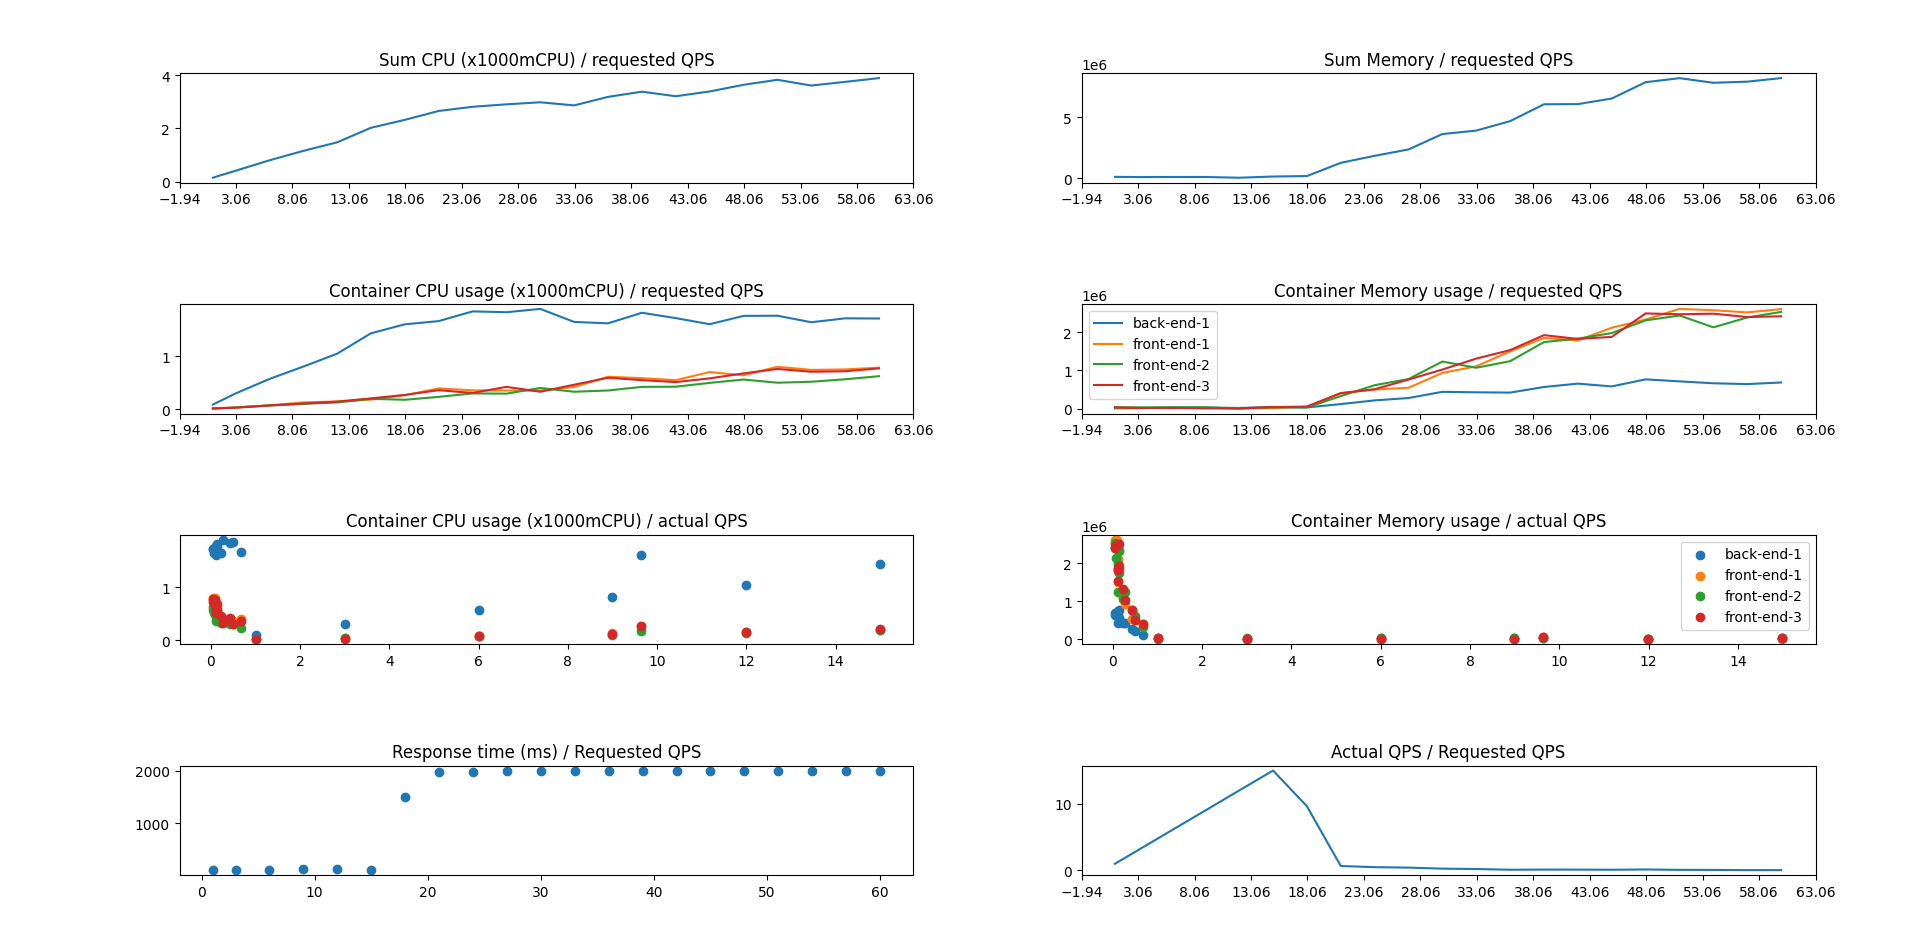
\includegraphics[width=150mm, keepaspectratio]{figures/taildrop-chain-3FE-1BE_requestedQPS.png}
	\caption{Három költséghatékony frontend után egy költséges backend mérés ábrázolása}
	\label{fig:3FE_1BE_chain}
\end{figure}

\subsection{Költséghatékony frontendek egymás mellett és költséges backend mögöttük}
%----------------------------------------------------------------------------
\Aref{subsec:3FE_1BE_chain} fejezetben bemutatott tapasztalatokat igazoló, készítettem egy következő mérést is. Ebben az esetben kicsit egyszerűbb architektúrával végeztem el a mérést. A megkonstruált erőforráshasználatok és a rendszer felépítését táblázatos formában \aref{tab:3FE_1BE_new} táblázat tartalmazza.

Fontos különbség, hogy ebben a mérésben nem hozunk létre egy hosszú láncot az egyes frontend alkalmazások egymás mögé kötésével, hanem ennél sokkal rövidebb lesz egy-egy kérés kiszolgálásának folyamata. 
A költséghatékony frontend után rögtön a költséges backendhez kerül továbbításra a beérkező kérés.
Ezen kívül még egy fontos módosítás, hogy három darab frontend fog futni és továbbra is egy backend lesz hátul.
A megadott alapján kiszámolható az egyes egységek által körülbelül kiszolgálható kérések száma másodpercenként.
\refstruc{eq:3FEsumqps} alapján leolvasható, hogy a \textit{front-end-1} áteresztő képessége 120 kérés, míg a \textit{back-end-1} ennél jóval szerényebb 20 beérkező kérést tud kiszolgálni másodpercenként, mint ahogy az következik \aref{eq:1BEsumqps} egyenletből.

\begin{equation}
\label{eq:3FEsumqps}
3(replika)\times\frac{1000 mCPU}{25 mCPU/kérés} = 120 kérés/másodperc
\end{equation}

\begin{equation}
\label{eq:1BEsumqps}
1(replika)\times\frac{2000 mCPU}{100 mCPU/kérés} = 20 kérés/másodperc
\end{equation}

\begin{table}[]
\centering
\begin{tabular}{l|ll}
Név                                                            & front-end-1   & back-end-1 \\ \hline
Replikák száma                                                 & 3             & 1          \\
\begin{tabular}[c]{@{}l@{}}CPU használat\\ (mCPU)\end{tabular} & 25            & 100        \\
\begin{tabular}[c]{@{}l@{}}CPU limit\\ (mCPU)\end{tabular}     & 1000          & 2000       \\
\begin{tabular}[c]{@{}l@{}}Memória limit\\ (kB)\end{tabular}   & 1000          & 1000       \\
Továbbhívás                                                    & back-end-1:80 & -          \\
HPA                                                            & -             & -         
\end{tabular}
  	\caption{Költséghatékony frontend több replikával és utána egy költséges backend}
	\label{tab:3FE_1BE_new}
\end{table}

Jelen mérésben nincsen megadva semmilyen automatikus skálázó, ezért amikor az operátor az indításkor létrehozza adott replikaszámmal az egyes Kubernetes Deploymenteket, azok nem is fognak változni, függetlenül a beérkező kérések mennyiségétől.
A korábban bemutatott környezeten is elvégeztem a szimulált terheléssel történő mérést.
Ezen eredményeket mutatja be \aref{fig:3FE_stack_1BE} ábra.
A korábbi méréssel szinkronban, hasonló megállapításokat tudunk leolvasni.
Látható, hogy a \textit{back-end-1} telítése az elvárt 20 QPS körül megtörténik (illetve kicsit még előtte). 
Azonban ettől függetlenül a \textit{front-end-1} által elhasznált processzor mennyisége folyamatosan nőtt. A legmagasabb terhelésnél már olyan szintre emelkedett a három példány által összesen használt processzor erőforrása, mint a backend maximuma, tehát mintha 2 teljes virtuális CPU magot is allokáltunk volna számukra.

A költséges backend telítése után jelentősen megugrik a beérkező kérések kiszolgálásához szükséges késleltetések és az egyes egységek által használt memória mennyiségek is.
A jobb alsó grafikonon látszik, hogy 20 QPS-nél már vissza is zuhant a sikeres kiszolgálások száma, amivel szinkronban a kiszolgálások átlagos válaszideje is felurik a maximumra, ami jelenleg 5 másodperc, mert a beállítások szerint ennyi idő után bontjuk a \textit{http} kapcsolatokat.

\begin{figure}[!ht]
	\centering
	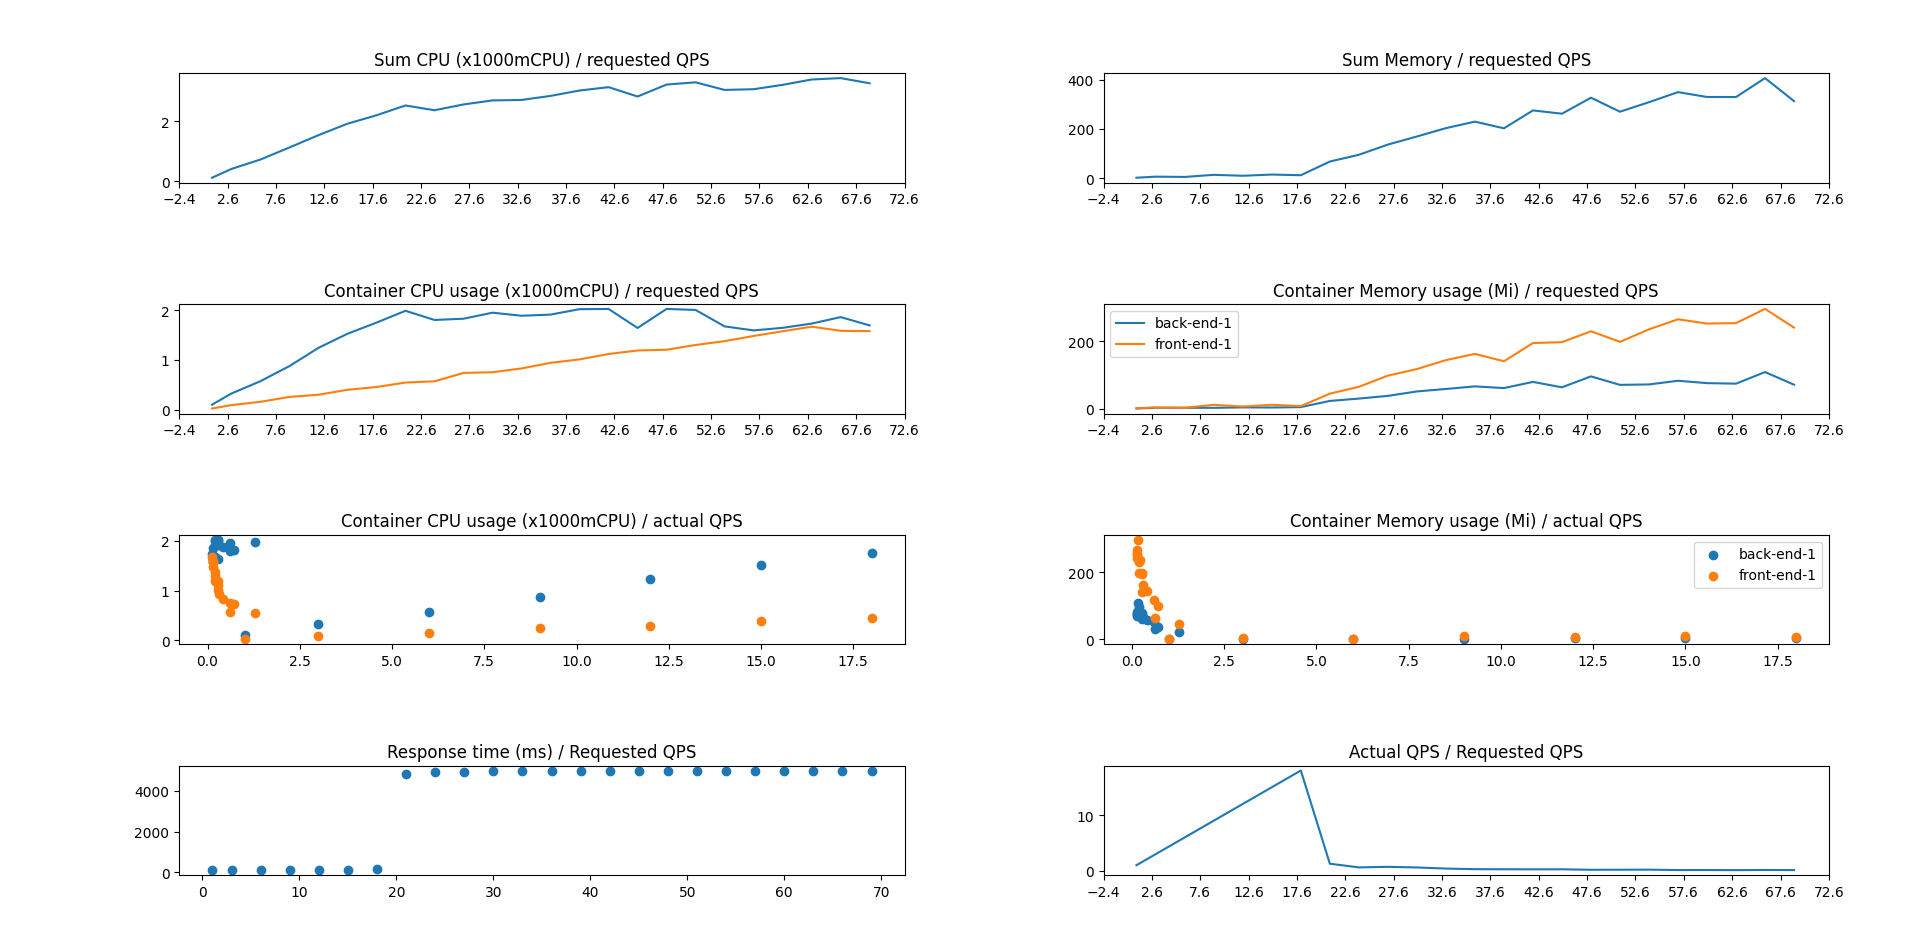
\includegraphics[width=150mm, keepaspectratio]{figures/multiFE-singleBE.png}
	\caption{Költséghatékony frontend három példányban és utána egy költséges backend mérés ábrázolása}
	\label{fig:3FE_stack_1BE}
\end{figure}

Röviden elmondható, hogy a beérkező kérések növekedésével együtt fokozatosan nő az elhasznált processzor mennyisége és a sikeres kiszolgálások száma is.
Azonban van egy pont, amikor a hálózatban lévő szűk keresztmetszet nem képes tartani a lépést a beérkező kérések mennyiségével. 
Ebben az esetben hirtelen visszaesik a kiszolgálás minősége, drasztikusan megugrik a várható kiszolgálási idő és ezzel együtt csökken a sikeres kiszolgálások aránya.

Az elvégzett mérések esetén látható, hogy valódi problémáról van szó, abban az esetben, ha a rendszer az előre definiált erőforráshasználatokkal fut és nem képes azokat automatikusan állítani.
Ha a beállítások dinamikusabbak lennének, akkor például a frontend által lefoglalt és használt erőforrásokat át lehetne csoportosítani a backend részére, amivel növelhető lenne a rendszer globális maximum kiszolgálása.

%----------------------------------------------------------------------------
\section{Mérések automatikus horizontális skálázóval}
%----------------------------------------------------------------------------

A korábban végzett mérések alapján ki lehet jelenteni, hogy a podok statikus konfigurálásával nem mindig találjuk meg a rendszer ideális állapotát,  sőt a jövőbeli terhelés pontos információja nélkül nagyon valószínű, hogy szuboptimális állapotban maradunk.
A Kubernetes beépítetten támogatja a podok automatikus horizontális skálázását, mint ahogy azt \aref{subsec:hpa} alfejezetben bemutatásra került.
A további haladás részeként szerettem volna megnézni, hogy milyen megoldást kínál beépített skálázó és mik a limitációi.
A fő cél az volt, hogy bizonyítást nyerjen, hogy a skálázó algoritmusa miatt nem képes minden esetben egy ideális állapotba jutni.

\subsection{Áttérés nehézségei}
%----------------------------------------------------------------------------

Az új fajta mérés több gondot is okozott, tekintve hogy az eddigre bejáratott ábrázoló alkalmazást teljesen át kellett variálni, ugyanis ezen mérések jelentősen mások.
Ebben az esetben az egyes értékek az időtől változóan függnek, ellentétben a HPA nélküli méréseknél, amikor minden a beérkező terheléstől változott. Valamint a kezdeti méréseknél kiderült, hogy az elkészített operátor logikai működésében is hiba van. 
A jelenség onnan fakadt, hogy minden egyes alkalommal, amikor az operátorunk futásra került, ellenőrizte a ServiceGraph konfigurációban megadott replika számot és ha nem stimmelt, akkor módosította azt.
Ezen logika miatt, amikor a skálázó szeretett volna több azonos podot elindítani egy adott alkalmazásból, akkor ezt észrevette az operátor és visszaállította a kezdeti értéket.
A következmény pedig az lett, hogy a rendszer sosem került stabil állapotba és skálázó döntései nem tudtak érvényre jutni.

A fenti probléma ideálisan példaként tud szolgálni az operátorok egy kevésbé kutatott és ritkán tárgyalt kihívására.
Amennyiben több kezelő alá esik egy-egy Kubernetes erőforrás, akkor nagyon körültekintően kell eljárni az egyes feladatkörök elosztásában.
Nem triviális észrevenni, ha direkt vagy indirekt módon, egymás döntéseire reagáltan futnak le az operátorok algoritmusai.
Ezzel a rendszer egésze könnyen instabil vagy holtponti (deadlock) állapotba tud kerülni.

Egy-egy ilyen helyzetet felismerni aránylag körülményes, alapértelmezetten nincsen erre külön logika implementálva az orkesztrációs platformba.
Emiatt ezen esetek detektálása, újabb operátor bevonása nélkül nem lehetséges.
Azonban újabb logika bevonása, ami azonos erőforrások kezelését teszi lehetővé, tovább növelheti az indirekt egymásrahatások valószínűségét.

Természetesen a fenti probléma könnyen javíthatónak bizonyult és csak egy kisebb módosításra volt szükség.
Végleges implementációban a megadott replikaszám ellenőrzése az egyes deploymentekben csak akkor kerül ellenőrzésre, ha autómatikus skálázó nem került definiálásra a megadott konfiguráció alapján.

\subsection{Lokálisan mohó, globálisan nem optimális}
%----------------------------------------------------------------------------

% TODO: x. fejezetben bemutatott
A HPA skálázó döntési mechanizmusát ismerve, sejthető volt, hogy milyen szituációkra viselkedhet érzékenyen.
Maga az algoritmus, ami meghatározza az egyes podokból aktuálisan szükséges darabszámot egyedül az ő feleőssége alá tartozó konténereket veszi számításba.
Ezen kívül nem rendelkezik egyéb ismerettel a többi szolgáltatást illetően.
Például nem tudja, hogy milyen más alklamazás komponensekkel van kapcsolatba az alá tartozó komponens se azt, hogy mennyi erőforrás érhető el összesen a klaszterben.

A fenti tulajdonságok alapján a jelenlegi skálázó csak lokálisan optimális döntéseket tud hozni egy-egy alkalmazás egység számára.
Azt kellett bebizonyítani, hogy ezen tulajdonsága miatt a rendszer összeségét érintő, globális optimumot nem fogja megtalálni.
Ehhez létrehoztam egy egyszerű szolgáltatás hálót és az egyes elemekhez tartozó horizontális skálázót. 
A konkrét értékeket \aref{tab:1FE_1BE_chain_with_HPA} táblázat tartalmazza.
Látható, hogy a korábbi mérésekhez hasonlóan itt is egy Frontend és egy Backend alkalmazás szerepel. 
A kérések a frontendhez érkeznek be, ami mindegyiket továbbítja a backend felé. 
Az egyes komponens podok által lefoglalt és maximálisan használható erőforrások mennyisége megegyezik.
Egy virtuális CPU magot használhatnak illetve egy megabájt memóriát.
Annyi különbség van, hogy a frontend a beérkező kérésenként negyed annyi CPU használatot fog generálni, mint a backend.

A korábbi mérésektől eltérően ebben az esetben az operátorunk a konfiguráció alapján fog létrehozni automatikus horizontális skálázót is.
Azonos szabályok kerültek alkalmazásra a két egységhez kapcsolódóan.
Legalább egy podnak futnia kell de legfeljebb öt futhat egyszerre, illetve a processzor használtságot figyelembe véve fogjuk meghozni a skálázási döntést.
Ebben az esetben a HPA törekedni fog a 70 százalékos foglaltságra. 
Tehát a maximálisan elérhető proszeszor használat 70 százaléknál magasabb használata esetén fogjuk megkezdeni a felskálázást.

\begin{table}[]
\centering
\begin{tabular}{ll|ll}
\multicolumn{2}{l|}{Név}                                                                      & front-end-1   & back-end-1 \\ \hline
\multicolumn{2}{l|}{Kezdeti replika szám}                                                     & 1             & 1          \\
\multicolumn{2}{l|}{\begin{tabular}[c]{@{}l@{}}CPU használat\\ (mCPU)\end{tabular}}           & 25            & 100        \\
\multicolumn{2}{l|}{\begin{tabular}[c]{@{}l@{}}CPU foglalás és limit\\ (mCPU)\end{tabular}}   & 1000          & 1000       \\
\multicolumn{2}{l|}{\begin{tabular}[c]{@{}l@{}}Memória foglalás és limit\\ (kB)\end{tabular}} & 1000          & 1000       \\
\multicolumn{2}{l|}{Továbbhívás}                                                              & back-end-1:80 & -          \\
\multirow{3}{*}{HPA}                            & Minimum replika                             & 1             & 1          \\
                                                & Maximum replika                             & 5             & 5          \\
                                                & Cél CPU használat                           & 70\%          & 70\%      
\end{tabular}
\caption{Három költséghatékony frontend után egy költséges backend}
\label{tab:1FE_1BE_chain_with_HPA}
\end{table}

A generált terhelés hatására a rendszernek másodpercenként hetven beérkező kérést kellett kiszolgálnia. 
Az egyes http kapcsolatokra a megszokott módon öt másodperces időkorlát volt, amin belül ha nem érkezett válasz, akkor az adott kérést sikertelennek tekintjük.
A teljes szimuláció a szolgáltatásháló létrehozásától számított tíz percig, azaz hatszáz másodpercig tartott.

Mérés során parancssorból is jól látható a skálázó működése. 
Ezt mutatja be \aref{hpa_measurement_pending} kódrészlet, amin belül két paranccs kimenetét is láthatjuk a mérés kezdetét követő bő öt és feledik percben.
Első sorban lekérdezzük az éppen működésben lévő horizontális skálázókat. 
A parancs kimenetének második oszlopából kiderül, hogy az egyes skálázók az azonos névvel rendelkező deployment erőforráshoz vannak kapcsolva.
Leolvasható, hogy skálázó döntései alapján öt és négy replikának kellene futni ebben az időpillanatban illetve, hogy mind a frontend mind pedig a backend túl lépte a számára előirányzott processor fogyasztást.

A kódrészlet második parancsán láthatjuk, hogy milyen podok és milyen állapotban léteztek ilyenkor.
Megfigyelhető, hogy valóban szerepel a korábban a skálázó által meghatározásra kerülő négy darab frontend és az öt darab backend kapszula.
Viszont, ami tanulságos, hogy közüllük nem mindegyiknek sikerült az elvárt módon elindulnia.
Erre abból lehet következtetni, hogy egyes podok állapot mezője nem az elvárt \textit{Running}, hanem \textit{Pending} állapotban vannak.
Amiatt van ez, mert ugyan a skálázó döntése alapján el kellene induljon az elvárt számú kapszula, azonban a Kubernetes ütemezője nem tudja őket elindítani.
Látható, hogy három plusz három kapszula tudott rendesen elindulni, így rögtön hat virtuális cpu magot le is foglaltunk a klaszterben és nem tud új egységet lehelyezni.
Ez a magyarázata, hogy míg a korábban elindított egységek (magasabb \textit{AGE} értékkel) sikeresen elindultak, azonban a későbbieknél ez már nem mondható el.

% HPA bekapcsolva, nem ideális eredmény ----------------------------------------
\lstset{caption=Horizontális skálázóval történő mérés, label=hpa_measurement_pending}
\lstinputlisting{figures/HPA-pending-pods.sh}

A mérés eredményeit ábrázolva előkerült egy érdekesség is, amit \aref{fig:HPA-scaling-same-time} ábrán láthatunk.
A grafikonon egyszerre van ábázolva a frontendből és a backendből futó egységek száma is.
Erre utal a bal felső sarokban szereplő jelmagyarázat is, viszont a kék színnel rajzolt költségesebb backend nem is látszik.
Ez amiatt van, mert a Prometheus adatai szerint egyszerre történtek meg a skálázások és ez az oka, hogy mindkét alkalmazásegységből három, három darab került elindításra.
Értelemszerűen ez az erőforrások nem ideális elosztását vonja magával, hiszen azonos erőforrás került lefoglalásra és használatra a költségesebb illetve könyebb alkalmazásrész részére is.
Ha a skálázó rendelkezne a környezetéről több inforációval, akkor ennél ideálisabb arányban tudna erőforrásokat allokálni.
Például, ha feltesszük, hogy összesen hat pod indítható, akkor előnyösebb lenne egy 2-4 vagy 1-5 megosztás a költségesebb backend javára.
Viszont a tapasztalható megosztással nem tudjuk maximálisan kihasználni a rendszerben lévő erőforrásokat.
Pontosabban mondva kihasználjuk, mert a lefoglalt processzor mennyiségét jelentősen kihasználjuk, azoban a kiszolgálás minősőgén és mennyiségén ez nem látszódik.

\begin{figure}[!ht]
	\centering
	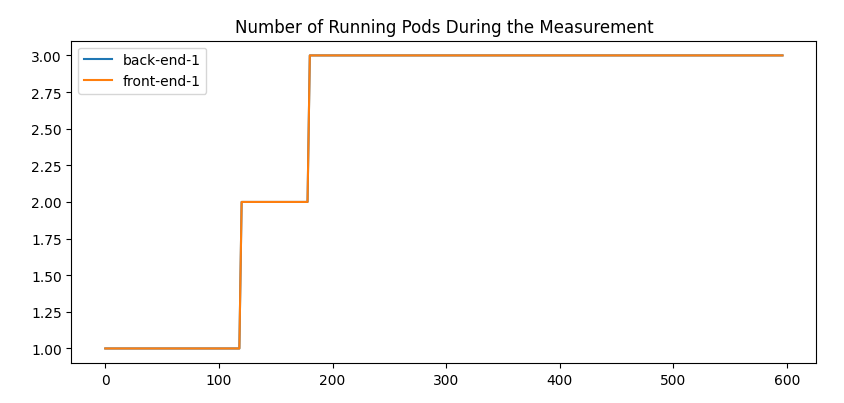
\includegraphics[width=150mm, keepaspectratio]{figures/HPA-scaling-in-the-same-time.png}
	\caption{HPA skálázóval történő mérés}
	\label{fig:HPA-scaling-same-time}
\end{figure}


%----------------------------------------------------------------------------
\chapter{Megoldási lehetőségek}
\label{sec:solutions}
%----------------------------------------------------------------------------

Ebben a fejezetben szeretném bemutatni, hogy a korábban \aref{sec:results} fejezetben látott mérések alapján milyen megoldási lehetőségek jöhetnek számításba.
Természetesen minden bemutatott megoldásnak megvan a saját erőssége és gyengesége, amiket a következő alfejezetben részletesen is ismertetek.

%----------------------------------------------------------------------------
\section{Feltárt probléma rövid összefoglalása}
%----------------------------------------------------------------------------

A megoldási lehetőségek bemutatása előtt szeretném röviden összefoglani a problémát és felvetést, amire keressük a megoldást.
A mérési eredmények alapján arra jutottam, hogy léteznek olyan skálázási helyzetek, amikor a Kubernetes jelenlegi skálázója nem tud ideálisan lekezelni.
Ez a működés onnan fakad, hogy a futó alkalmazásról nem rendelkezik globális ismerettel, csak az egyes független szolgáltatásokat kezeli a többitől függetlenül.

A látott mérésekből kiderült, hogy a jelenlegi rendszerben létezik egy átbukási pont, amikor a beérkező kéréseket az össz alkalmazás már nem képes időben kiszolgálni, mert az egyik szolgáltatási komponens túlterhelt állapotba kerül.
Ilyenkor a beérkező kérések továbbra is fogadásra kerülnek és elkezdődnek a bufferek megtöltései a rendszerben.
Ez egy öngerjesztő folyamatot indít meg, ahol a hosszabb sorbanállás, a folyamatos túlterheltség miatt aránylag egyre kisebb lesz a sikeres kiszolgálások száma. 

A hatékonytalan működésen az sem segít, hogy az előre beállított idő túllépése után bontjuk a kapcsolatot, azonban ezt az alklamazás nem tudja lekezelni.
Nem létezik implementált megoldás arra az esetre, hogy az ilyen kérések által keltett az egyéb alkalmazás egységek terhelését megszüntesse.
Értelemszerűen ebben az esetben felesleges még a back-end oldalán elvégezni az erőforrás intenzív feladatot, amikor az azt kiváltó eredeti kérés eldobásra került.

A feltárt problémát két részre lehet osztani, amik egymás hatását tudják erősíteni vagy gyengíteni.

%----------------------------------------------------------------------------
\section{Lehetséges eszközök}
%----------------------------------------------------------------------------

A kiírásban megfogalmazott feladatom volt, hogy keressek olyan kiegészítést vagy javaslatot, ami a jelenlegi HPA működését javítani tudná.
A feladatom elvégzése és források keresése közben számos megoldási lehetőség felmerült.
A bemutatott eszközök elemzése során látni fogjuk, hogy kicsit más megközelítésből és a probléma más aspektusát célozva próbálja a feltárt hatásokat csökkenteni.

Az egyes eszközök értékelésénél az is fontos szempont volt, hogy a lehető legkevesebb módosítást kelljen végrehajtani az alkalmazás oldalán.
Ez fontos, mert a megvalósítani kívánt feladat nem tartozik szorosan az alkalmazáshoz és ideális esetben teljesen transzparens módon működne.
Természetesen több dolgot is mérlegelni kell az adott helyzetben ideálisnak itélt megoldás kiválasztása közben.

Fontos azt is megfontolni, hogy egy az infrastruktúrális részekre hatást gyakorló eszköz milyen információk alapján engedjük, hogy dolgozzon.
Természetesen minél több információval rendelkezünk az adott alkalmazást illetően, annál optimálisabb megoldásokat tudunk adni.
Például, ha egy okos skálázónak rálátást adunk az alkalmazás hálózatára, az egyes egységek által használt erőforrásokra, a köztük lévő kapcsolatra és esetleg saját metrikákat is kivezetünk, akkor a skálázási döntés meghozatalában ezeket mind számításba tudjuk venni.
Másik oldaról viszont aggályos lehet, ha ilyen szintű monitorozást és belelátást biztosítunk, mert ezáltal következtetéseket tudunk levonni a futtatott alkalmazásról.
Ez pedig bizonyos esetekben az ügyfél érdekeit sértheti.


\subsection{Beépített állapotjelzők}
%----------------------------------------------------------------------------
A Kubernetes kapszulák létrehozása közben, beépített módon lehetőségünk van a kapszula állapotáról jelzési pontokat meghatározni.
Ezzel a megoldással sokrétűen használható funkciókat kapunk, amivel közvetetten több dolog befolyásolására nyílik lehetőségünk.
Három jelzési módszerünk van, amit három különböző esetre találtak ki.
Az alapvető felvetés onnan fakad, hogy különböző, gyakran előforduló helyzetekre adnak megoldási lehetőségeket különálló működésük által.
Az egyes állapotjelzők ideális használati módját az alábbi szituációkkal szeretném szemléltetni.

\begin{enumerate}
    \item \textbf{(Liveness probe - életteli próba)} Előfordulhat, hogy az alkalmazásunk valamilyen bemenetek következtében holtponti állapotba kerül, amit nehéz lenne kívülről észrevenni, viszont külső behatás nélkül nem tudna továbblépni belőle. 
    Illetve egyéb okok miatt is kerülhet olyan állapotban, amikor a vizsgált alkalmazás nem képes ellátni a működését, mindezt különösebb hiba és kilépés nélkül teszi.
    Szerencsére az ilyen esetek nem számítanak különösnek és hamar fel is lehet oldani az egység újraindításával, amit az életteli próbával tudunk kezelni.
    Ez egy teljesen ideális implementció esetén nem fog gondot okozni, hiszen a kapszulák nem tartalmaznak, tárolnak fontos adatokat és állapotokat.
    Egy újraindítás sokkal idő- és költséghatékonyabb megoldás, mintha az egész rendszer funkcionális működését veszélyeztetnénk.

    \item \textbf{(Startup probe - indítási próba)} Eshetőség, hogy az alkalmazás elindítása után még el kell végezni pár inicializációt, mielőtt a külső kérések kiszolgálását elkezdhetné.
    Ebben az esetben is tudatni kell az infrastruktúra részére, hogy a jelenlegi állapotába még nem áll készen a működésre.
    Nagy hibázási lehetőséget rejtene magába, ha erre a korábban látott  életteli próbát használjuk, mert nehéz kiszámítani mennyi időt fog igénybevenni a komponens elindulása.
    Külön emiatt létezik az indítási próba, ami csak akkor fogja az adott kapszula állapotát készenléti státuszba sorolni, ha sikeresen lefutott a próba.

    \item \textbf{(Readiness probe - készenléti próba)} Tegyük fel, hogy van egy szolgáltatásunk, ahol nagy fájlok feltöltésére van lehetőségünk.
    A megvalósított funkció szám
    Ez egy időigényesebb feladat lesz, miközben az alkalmazásunkat nem szeretnénk további kérésekkel terhelni.
    Ebben az esetben meg kell várni a korábban érkező kérés kiszolgálását és csak utána van lehetőségünk fogadni a többit.
    Ilyen helyzetben tudjuk használni a készenléti próba jelzést. 
    Amennyiben a próba sikertelen vol, tehát jelenleg nem engedhetünk új kiszolgálást, akkor a kapszula IP címe ki fog kerülni erre az időszakra a hozzá tartozó \textit{Service} alól, így forgalom se fog eljutni hozzá. 
    
\end{enumerate}

A fentebb bemutatott eszközök megkönnyítik a robosztus rendszerek építését.
Segítségükkel kihasználhatjuk, hogy inkább az előforduló hiba gyors észrevételét és nem annak az elkerülését részesíti előnyben.
Erre lehetőség is van, mert az új konténerek elindítása általában pár másodperc alatt megtörténik és ezáltal egy öngyógyító tulajdonsággal is fog bírni a kész rendszer.
Így pedig a rendszer megbízhatósága is javulni fog. 

Ennek ellenére körültekintően kell ezeket az eszközöket is használni, hiszen rossz konfiguráció esetén mi magunk tehetjük működésképtelenné a rendszert.
Például, hibás beállítás esetén az életteli próba hajlamos állandóan újraindítani az alkalmazást. Vagy a készenléti próba miatt egyes komponens egységek nem fognak annyi kérést kapni, amit azok valóban képesek lennének kiszolgálni.

\subsection{Konténer specifikus metrikák alapján}
\label{subsec:container_metric_scaling}
%----------------------------------------------------------------------------
Következőnek ismertetett megoldási javaslat szintén a beépített Kubernetes erőforrásokat és azok funkcióit kívánja felhasználni.
Ezen megoldásoknak előnye, hogy a klaszter oldaláról nem igényelnek nagy mértékű többlet fejlesztést és támogatást, hiszen ezek a funkciók valószínűleg rendelkezésre állnak már a rendszerben vagy pedig könnyen telepíthetőek.
A mérleg másik oldalán ezen megoldások az alkalmazás oldalán igényelnek fejlesztéseket vagy pedig a helyes konfiguráció okozhet kihívást.

Még korábban, \aref{subsec:hpa} alfejezetben bemutatott HPA skálázás esetén említésre került, hogy tetszőleges metrikák alapján is lehetőségünk van skálázni.
Alapértelmezetten és leginkább a mérések által általunk is használt processzor erőforrás igény alapján történő skálázás a legelterjedtebb forgatókönyv.
Ezen metrikákat a klaszter automatikusan tudja gyűjteni, így a skálázók konfigurációja és elindítása egyszerű folyamattá tud válni.
Illetve a legtöbb esetben, ha a klaszterünkben nincsenek szűkös erőforráshatárok aránylag jó működést eredményez.




\subsection{Service Mesh}
%----------------------------------------------------------------------------

\subsection{Gloo Edge}
%----------------------------------------------------------------------------

\subsection{Okos skálázó}
%----------------------------------------------------------------------------

A korábban bemutatott megoldási lehetőségeknél, \ref{subsec:container_metric_scaling} alfejezetben látottat leszámítva, a fő motiváció a beérkező terhelés szabályozása volt.
Az eredeti problémánkat viszont több irányból is meg lehet fogni.
Másik megközelítésben az erőforrások globálisan optimális elosztása a fő szempont a megoldandó kihívás.

A következő megoldási javaslat ezt a megközelítést veszi alapul és bővíti ki a korábban látott javaslatokkal.
A javaslat egy központi skálázó alkalmazás, ami folyamatosan monitorozza a klaszter teljes állapotát és az éppen futtatott alkalmazásokat is.
A skálázási javaslatokat pedig ezen információk összeségéből tudja meghatározni.
Így figyelembe tudja venni az egyes kapszulák minőségi osztály besorolásuktól kezdve az egyes komponensek közti forgalmak megosztásán keresztül az esetlegesen exportált alkalmazás metrikákig.



Namespacek között

fejlesztés, tesztelés

pl: nyomon követi milyen arányban használják az erőforrásokat

Amdahl's törvényt is figyelembe  veszi
VPA és HPA együtt működik
%----------------------------------------------------------------------------
\chapter{Összefoglalás}
\label{sec:summary}
%----------------------------------------------------------------------------


%----------------------------------------------------------------------------
\section{Elvégzett munka}
%----------------------------------------------------------------------------
%Alapvetően jól működik a beépített skálázó.
%Pár extra lépéssel javítható lenne.
%Vagy nagyon komplex lehetőség vezetne csak sikerre.

Szeretném röviden összefoglalni a diplomamunkában tárgyalásra kerülteket és ezáltal az elvégzett munkát is, hogy a korábban végigvezetett gondolatmenet részei egészben is megjelenjenek.

A fő vizsgálandó terület a terhelésfüggő HPA skálázó működése volt szolgáltatáshálókon.
Ez a kérdés egyre több ágazatot érint, ahogy egyre többen választják az alkalmazásaik futtatására a felhőt, mint platformot.
Bevezetésként felvázoltam ezen folyamatot, annak beazonosítható elemeit és a jelenlegi tendenciákat.

Ezután a technikai részletek és megvalósítás előtt bemutattam a diplomadolgozat központi szerepét játszó Kubernetes klaszter felépítést, és a benne elérhető erőforrások szabályozását és a beépített skálázóját.

Az érdemi feladatok előtt fel kellett mérni a szakmán belül elérhető korábbi kutatásokat. Ismertettem a főbb elméleti vonalakat és ötleteket gyűjtöttem a saját munkához.

A kérdések megválaszolásához sok mérést kellett végezni, melyhez nélkülözhetetlen volt implementálni egy erre alkalmas környezetet. 
A környezet több különálló részből állt.
Létre kellett hozni egy saját erőforrást a Kubernetesen belül és implementálni egy kezelő logikát hozzá.
Szükség volt egy tetszőlegesen konfigurálható alkalmazásra, ami előre beállított végpontokra érkező kéréseket szolgál ki.
A mérés vezénylését és a kapott eredmények megjelenítését egy-egy külön alklmazás végzi.

Méréseken keresztül először megismertük, hogyan viselkednek a szolgáltatáshálók forgalomszabályozás nélkül egy túlterhelt rendszerben. 
Láttuk, hogy egy átbukási pont után a kiszolgálási paraméterek nagymértékben visszaesnek.

Következő kérdés, amire válasz született, hogy ezeket az eseteket mennyire csillapítja a HPA.
Láthattuk, hogy szűkös erőforrások esetén nem minden esetben sikerül elérni az elméleti optimum pontot, és a végeredmény függ a rendszer eredeti állapotától és a jól eltalált konfigurációtól.
Amennyiben kellően nagy mennyiségű erőforrás áll rendelkezésre, akkor a HPA képes lenne a lokálisan optimális döntések által mindig növelve a szűk keresztmetszetet, egy globálisan is elfogadható állapotba kerülni.

A szolgáltatáshálók és a skálázó esetében megfigyelt limitációkra több megoldási javaslatot is adtam, melyek a probléma más-más aspektusát megragadva próbálják megszüntetni vagy csökkenteni azt.
Ezen javaslatoknál bemutatásra került az adott eszköz előnye és hátránya is, hogy megfontoltabb döntési alapot kínáljon.

%----------------------------------------------------------------------------
\section{Dolgozatban nem vizsgált kérdések}
%----------------------------------------------------------------------------
A diplomamunka keretén belül sikerült elmélyülni a feladatban, miközben folyamatosan bontakozott ki a terület komplexitása.
Sok feladatot sikerült megvalósítani és a legtöbb vizsgált kérdésre sikerült választ is kapni azonban a tanulmányok során tetemes számban kerültek elő olyan kérdések, amik a rendelkezésre álló idő miatt nem sikerült felderíteni.
Ezen kérdéskörök további vizsgálatot és kutatást igényelnek.

Az elvégzett mérések során bizonyos egyszerűsítésekkel éltem, hogy értelmezhető maradjon a kapott eredmény.
Ilyen egyszerűsítés például az a megkötés, hogy a beérkező kérések száma egyenletes az időben, azonban ez nem minden rendszer esetén van így.
Jól megfigyelhető periódusok jelentkezhetnek egy napon, hónapon vagy éven belül is.
Több projekt is foglalkozik ezzel a jelenséggel és próbálják szintén keresni az erőforrások ideális használatát a historikus adatok elemzésével.
Létezik egy fejlesztés, ami a horizontális pod skálázót szeretné ilyen irányba továbbfejleszteni\citep{predictiveHPAGithub}.
A skálázó segítségével szintén érdemes lenne méréseket futtatni, azonban ennek előfeltétele, hogy dinamikusabban lehessen forgalmat generálni.
Például az időben változóan illetve ezeket több alkalmazásvégpont irányába küldeni.

A dolgozatban elkészített mérések mögötti szolgáltatás hálók a leggyakoribb, egyszerű eseteket fedték le.
Egy valódi mikroszolgáltatás architektúra ennél nagyságrendekkel több komponenssel rendelkezik, melyek közti kapcsolatok is összetettebbek.
Jelenlegi keretrendszert tovább lehetne fejleszteni, hogy a komponensekhez érkező kérések megadott arányok mellett kerüljenek egyik- vagy másik további komponenshez továbbküldésre.
Ezzel kicsit dinamikusabbá lehetne tenni a mostani rendszert, ami minden beérkező kérés esetén azonos kérés-válasz folyamatokat fogja elindítani.

További vizsgálandó kérdés, hogy a kapott eredmények más környezetben hogyan változnak meg.
Például, más eredmény jöhet ki, ha több csomóponttal, nagyobb terhelés mellett, nagyobb erőforrás felhasználással történnek a tesztek.
Sajnos az ilyen klaszterek bérlése drága különösen, hogy a méréseink szándékosan magas mennyiségű processzort használnak, ami alapja szokott lenni a bérelt infrastruktúra utáni számlázásnak.


\subsection{Keretrendszer további használata}
%----------------------------------------------------------------------------
Az elvégzett munka jelentős részét kitevő keretrendszer lehetőséget biztosít további felhasználásra is.
A diplomamunkán belül a feladata az volt, hogy fiktív paraméterekkel rendelkező szolgáltatás hálókat tudjunk elindítani és létrehozni.
Ezen kívül egy igazán hasznos felhasználási mód lehet, ha már létező, üzemelő hálózatokat szeretnénk klónozni.
Tehát létre tudunk hozni kisebb másolatokat az eredeti rendszerről, ami közel azonos kiszolgálási és erőforrás felhasználási paraméterekkel fog rendelkezni, mint a valódi.
Ezután lehetőségünk van fiktív fejlesztéseket végezni az egyes komponensek átkonfigurálásával és az így kapott rendszert tesztelni.
Ezáltal könnyebben lehet megalapozott döntéseket hozni, hogy az aktuális környezetben melyik szolgáltatást érdemes fejleszteni, melyikkel lehet érdemben befolyásolni az eredő nyereséget.

Továbbá az előzőleg bemutatott példán keresztül ki tudjuk próbálni az aktuális rendszerünket egy új környezetben is.
Mindezt úgy tudjuk megtenni, hogy az alkalmazás egységeket alkotó képfájlok mozgatása nem szükséges, ezáltal nem csak gyorsabb lesz a tesztelés, hanem nem kell újabb felek számára elérhetővé tenni a megírt állományokat.
Az így létrehozott mérések betekintést tudnak nyújtani, hogy egy esetleges infrastruktúra váltás milyen változásokkal jár a kiszolgálási paramétereket illetően.


% Acknowledgements
%~~~~~~~~~~~~~~~~~~~~~~~~~~~~~~~~~~~~~~~~~~~~~~~~~~~~~~~~~~~~~~~~~~~~~~~~~~~~~~~~~~~~~~
%----------------------------------------------------------------------------
\chapter*{\koszonetnyilvanitas}
\addcontentsline{toc}{chapter}{\koszonetnyilvanitas}
%----------------------------------------------------------------------------

% Gábornak: Sok segítség, nem csak a szakmára tanított felkészülni, hanem az életre.  
% Családnak: Pénz és idő
% Schönherz kollégium: egyetemi társaság, sok tanulás, VM-ek


Nehéz szavakba önteni a dolgozat készítése közben feltörő érzéseket.
Egyszerre van jelen a megkönyebbülés, a hála, az alkotás szeretete, a kielégíthetelen tudásvágy és az elmúlás is.
A diplomamunkám nem jöhetett volna létre számos támogatás nélkül, amit a körülöttem lévő emberek áldozatos munkájukból kaptam.
Szeretnék köszönetet mondani, hogy az egyetemen eltöltött időm alatt a legkülönfélébb területeken tudást és élményt tudtam gyűjteni.
%Érzem és tudom, hogy ezek által korábbi lényemhez képest több lettem és ezzekkel felvértezve a társadalomnak is hasznosabb tagja lehetek és szívből remélem, hogy többet tudok majd vissza is adni.

Szeretném külön kiemelni Dr. Rétvári Gábor konzulensemet, mivel az egyetemen végzett minden egyes projekttárgyat a felügyelete alatt készíthettem.
Szakmai tanácsaival mindig tovább tudta gurítani a megakadónak tűnő feladatokat és végig iránymutatással segítette, hogy ne vesszek el az egyes részletekben és tudatosította, hogy a nagyképet figyelve jelenleg hol tartok.
Mindezek már önmagukban köszönetet érdemelnek, de nem csak konzulensemmé vált Gábor, hanem a kötelező feladatokon túl mentorommá is.
Számíthattam rá, amikor az egyes feladatok nehézsége és nagysága miatt motivációmat vesztettem illetve egyedülálló személysége már önmagában motiváló.
Megmutatta, hogy egyenességgel, nyitottsággal és örök jókedvvel milyen szélessé nyilhat ki a világ.
Hálás vagyok érte, hogy együtt dolgozhattunk és tanulhattam tőle minden egyes konzultáció vagy találkozás alkalmával.

Köszönettel tartozom a családom támogatásáért, hogy egész életemben fontos szerepet szántak a taníttatásnak.
Tudom, hogy jelentős áldozatokkal járt ez a folyamat számukra is, de remélem sikerült a legjobban kihasználni az eddigi lehetőségeket és hosszútávon meg fog térülni.
Nekik köszönhetem, hogy támogatásukkal lehetőségem nyílt az egyetemi éveimet a kellő szabadsággal megélni, ezáltal is felfedezve illetve jobban megértve saját magam és a világ működését.

Végül pedig szeretném megemlíteni a Schönhez kollégium közösségét, ahol lehetőségem volt olyan dolgokat is kipróbálni, amik nem  közvetlenül a szakmához, hanem a tágabban értelemben vett élethez hasznos tapasztalatokkal szolgáltak.
Kipróbálhattam magam több csoport élén is, ezzel is tágítva a saját komfortzónám határát és ösztönöztek az alkotás és gondolkodás aktív folyamatára.
 

% List of Figures, Tables
%~~~~~~~~~~~~~~~~~~~~~~~~~~~~~~~~~~~~~~~~~~~~~~~~~~~~~~~~~~~~~~~~~~~~~~~~~~~~~~~~~~~~~~
%\listoffigures\addcontentsline{toc}{chapter}{\listfigurename}
%\listoftables\addcontentsline{toc}{chapter}{\listtablename}


% Bibliography
%~~~~~~~~~~~~~~~~~~~~~~~~~~~~~~~~~~~~~~~~~~~~~~~~~~~~~~~~~~~~~~~~~~~~~~~~~~~~~~~~~~~~~~
\addcontentsline{toc}{chapter}{Irodalomjegyzék}
\bibliographystyle{acm}
\bibliography{bib/thesis}

% Appendix
%~~~~~~~~~~~~~~~~~~~~~~~~~~~~~~~~~~~~~~~~~~~~~~~~~~~~~~~~~~~~~~~~~~~~~~~~~~~~~~~~~~~~~~
%%----------------------------------------------------------------------------
\appendix
%----------------------------------------------------------------------------
\chapter*{\fuggelek}\addcontentsline{toc}{chapter}{\fuggelek}
\setcounter{chapter}{\appendixnumber}
%\setcounter{equation}{0} % a fofejezet-szamlalo az angol ABC 6. betuje (F) lesz
\numberwithin{equation}{section}
\numberwithin{figure}{section}
\numberwithin{lstlisting}{section}
%\numberwithin{tabular}{section}

%----------------------------------------------------------------------------
\section{A TeXstudio felülete}
%----------------------------------------------------------------------------
\begin{figure}[!ht]
\centering
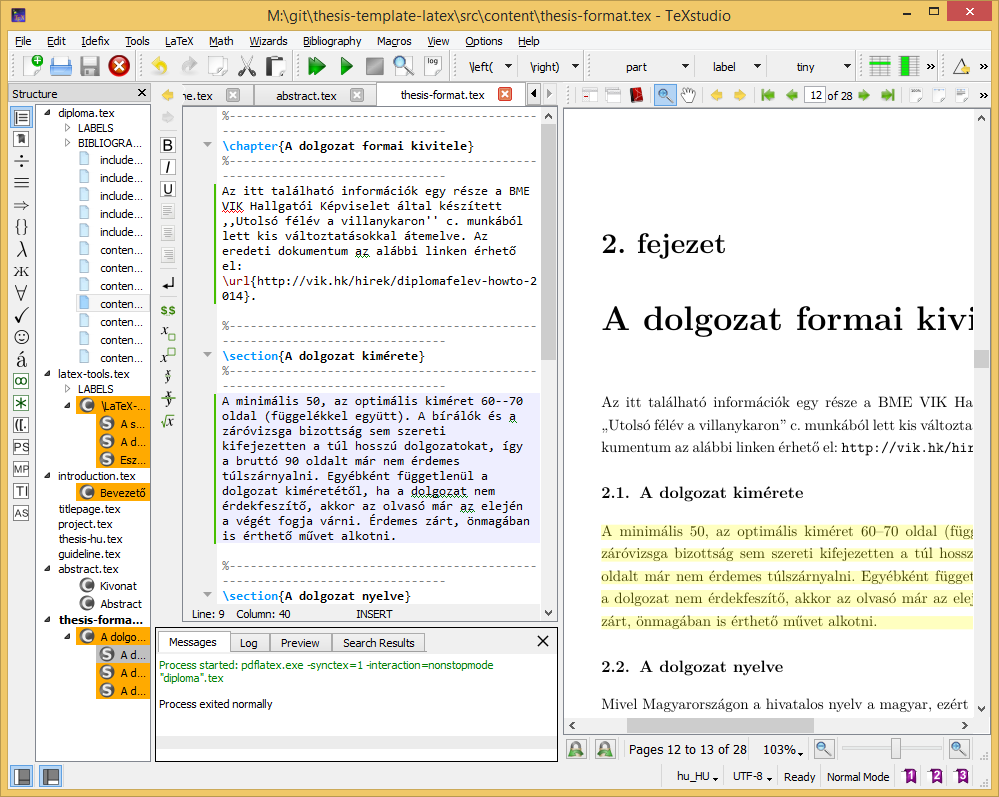
\includegraphics[width=150mm, keepaspectratio]{figures/TeXstudio.png}
\caption{A TeXstudio \LaTeX-szerkesztő.} 
\end{figure}

%----------------------------------------------------------------------------
\clearpage\section{Válasz az ,,Élet, a világmindenség, meg minden'' kérdésére}
%----------------------------------------------------------------------------
A Pitagorasz-tételből levezetve
\begin{align}
c^2=a^2+b^2=42.
\end{align}
A Faraday-indukciós törvényből levezetve
\begin{align}
\rot E=-\frac{dB}{dt}\hspace{1cm}\longrightarrow \hspace{1cm}
U_i=\oint\limits_\mathbf{L}{\mathbf{E}\mathbf{dl}}=-\frac{d}{dt}\int\limits_A{\mathbf{B}\mathbf{da}}=42.
\end{align}

%----------------------------------------------------------------------------
%\chapter{Rövidítések és fordítások}
\chapter*{Rövidítések és fordítások}
\label{sec:abbreviations}
\addcontentsline{toc}{chapter}{Rövidítések és fordítások}
%----------------------------------------------------------------------------

A szakterület sok rövidítést és mégtöbb angol kifejezést tartalmaz, amiket a lehetőségemhez mérten próbáltam magyarítani a könyebb olvashatóság érdekébe, illetve feloldani az első előfordulásakor.
Ahol találtam már előforduló magyar kifejezést, azt használtam, azonban az esetek nagy részében ez nem állt fent, így elnézést az esetlegesen váratlan és meglepő kifejezésekért.
Emiatt és a könyebb kereshetőség érdekében összegyűjtöttem a rövidítéseket és az általam használt magyarításokat.


\begin{multicols}{2}
\textbf{QPS} Queries per Second 

\textbf{HPA} Horizontal Pod Autoscaler / Automatikus Horizontális Pod Skálázó 

\textbf{VPA} Vertical Pod Autoscaler / Automatikus Vertikális Pod Skálázó 

\textbf{CPU} Processzor 

\textbf{I/O} Input and Output / Kimenet és Bemenet 

\textbf{K8s} Kubernetes 

\textbf{CNCF} Cloud Native Computing Foundation 

\textbf{Control plane} Vezérlő sík 

\textbf{Node} Csomópont 

\textbf{Pod} Kapszula 

\textbf{Kube Scheduler} Ütemező 

\textbf{CR} Custom Resource / Saját Erőforrás 

\textbf{CRD} Custom Resource Definition / Saját Erőforrás Leíró

\textbf{SLA} Service-level Agreement / szolgáltatási szint megállapodásokba

\textbf{QoE} Quality of Experience / érzékelhető szolgáltatási szint

\columnbreak

\textbf{API} Application Programming Interface / Alkalmazásprogramozási felület 

\textbf{OLM} Operator Lifecycle Manager / Operátor Életciklus kezelő 

\textbf{FE} Front-end 

\textbf{BE} Back-end 

\textbf{HTTP} Hypertext Transfer Protocol 

\textbf{Tight loop} Szoros ciklus 

\textbf{kubectl} Kubernetes parancssoros kezelője 

\textbf{Liveness probe} Életteli próba 

\textbf{Startup probe} Indítási próba 

\textbf{Readiness probe} Készenléti próba 

\textbf{Service Mesh} Szolgáltatás háló

\end{multicols}

%Todo
 % rövidítések, és fordítások

\label{page:last}
\end{document}
